% Seminar 12: Scoring models
% Statistics of Financial Markets -- Bachelor's programme, Bucharest University of Economic Studies
% GENERATED by latex/build_seminar12.py -- edit the generator, not this file.
% Student version by default; the instructor version is the *_solutions.tex wrapper.
\makeatletter\@ifundefined{ifsolutions}{\expandafter\newif\csname ifsolutions\endcsname}{}\makeatother

\newcommand{\coursename}{Statistics of Financial Markets}
% Preambul comun SFM -- Statistica piețelor financiare / Statistics of Financial Markets (Beamer, 16:9)
% Același design ca MFM. Înainte de % Preambul comun SFM -- Statistica piețelor financiare / Statistics of Financial Markets (Beamer, 16:9)
% Același design ca MFM. Înainte de % Preambul comun SFM -- Statistica piețelor financiare / Statistics of Financial Markets (Beamer, 16:9)
% Același design ca MFM. Înainte de \input{../../latex/preamble} se definește
%   \newcommand{\coursename}{Statistics of Financial Markets}      (EN)
%   \newcommand{\coursename}{Statistica piețelor financiare}       (RO)  și  \def\sfmlang{ro}
% Fișierele .tex se află în EN/Courses, EN/Seminars, RO/Cursuri, RO/Seminarii (două niveluri sub rădăcină).
% Deck-urile sînt generate de latex/build_chapterN.py / build_seminarN.py (vezi latex/sfm_build.py).

\documentclass[9pt, aspectratio=169, t]{beamer}
\providecommand{\coursename}{Statistics of Financial Markets}

% Ensure content fits on slides
\setbeamersize{text margin left=8mm, text margin right=8mm}

%=============================================================================
% THEME AND STYLE CONFIGURATION
%=============================================================================
\usetheme{default}
% Using default theme for clean header/footer control

% Color Palette (matching Redispatch PDF)
\definecolor{MainBlue}{RGB}{26, 58, 110}
\definecolor{AccentBlue}{RGB}{26, 58, 110}
\definecolor{IDAred}{RGB}{205, 0, 0}
\definecolor{DarkGray}{RGB}{51, 51, 51}
\definecolor{MediumGray}{RGB}{128, 128, 128}
\definecolor{LightGray}{RGB}{248, 248, 248}
\definecolor{VeryLightGray}{RGB}{235, 235, 235}
\definecolor{KeynoteGray}{RGB}{218, 218, 218}
\definecolor{SectionGray}{RGB}{120, 120, 120}
\definecolor{FooterGray}{RGB}{100, 100, 100}
\definecolor{Crimson}{RGB}{220, 53, 69}
\definecolor{Forest}{RGB}{46, 125, 50}
\definecolor{Amber}{RGB}{181, 133, 63}
\definecolor{Orange}{RGB}{230, 126, 34}
\definecolor{Purple}{RGB}{142, 68, 173}

% Gradient background (exact Keynote 315° gradient: white to RGB 218,218,218)
\setbeamertemplate{background}{%
    \begin{tikzpicture}[remember picture, overlay]
        \shade[shading=axis, shading angle=315,
        top color=white, bottom color=KeynoteGray]
        (current page.south west) rectangle (current page.north east);
    \end{tikzpicture}%
}
% Fallback solid color for compatibility
\setbeamercolor{background canvas}{bg=}

\setbeamercolor{palette primary}{bg=MainBlue, fg=white}
\setbeamercolor{palette secondary}{bg=MainBlue!85, fg=white}
\setbeamercolor{palette tertiary}{bg=MainBlue!70, fg=white}
\setbeamercolor{structure}{fg=MainBlue}
\setbeamercolor{title}{fg=IDAred}
\setbeamercolor{frametitle}{fg=IDAred, bg=}
\setbeamercolor{block title}{bg=MainBlue, fg=white}
\setbeamercolor{block body}{bg=VeryLightGray, fg=DarkGray}
\setbeamercolor{block title alerted}{bg=Crimson, fg=white}
\setbeamercolor{block body alerted}{bg=Crimson!8, fg=DarkGray}
\setbeamercolor{block title example}{bg=Forest, fg=white}
\setbeamercolor{block body example}{bg=Forest!8, fg=DarkGray}
\setbeamercolor{item}{fg=MainBlue}

% Footer colors (override Madrid theme blue)
\setbeamercolor{author in head/foot}{fg=FooterGray, bg=}
\setbeamercolor{title in head/foot}{fg=FooterGray, bg=}
\setbeamercolor{date in head/foot}{fg=FooterGray, bg=}
\setbeamercolor{section in head/foot}{fg=FooterGray, bg=}
\setbeamercolor{subsection in head/foot}{fg=FooterGray, bg=}

% Bullet styles (apply everywhere including blocks)
\setbeamertemplate{itemize item}{\color{MainBlue}$\boxdot$}
\setbeamertemplate{itemize subitem}{\color{MainBlue}$\blacktriangleright$}
\setbeamertemplate{itemize subsubitem}{\color{MainBlue}\tiny$\bullet$}
\setbeamertemplate{itemize/enumerate body begin}{\normalsize}
\setbeamertemplate{itemize/enumerate subbody begin}{\normalsize}

% Item spacing - compact style
\setlength{\leftmargini}{10pt}       % Level 1: minimal indent
\setlength{\leftmarginii}{10pt}      % Level 2: minimal additional indent
% Compact list spacing (zero extra space before/after lists in blocks)
\makeatletter
\def\@listi{\leftmargin\leftmargini \topsep 0pt \parsep 0pt \itemsep 0pt}
\def\@listii{\leftmargin\leftmarginii \topsep 0pt \parsep 0pt \itemsep 0pt}
\makeatother

\setbeamertemplate{navigation symbols}{}

%=============================================================================
% CUSTOM HEADLINE
%=============================================================================
\setbeamertemplate{headline}{%
    \vskip10pt%
    \hbox to \paperwidth{%
        \hskip0.5cm%
        {\small\color{FooterGray}\renewcommand{\hyperlink}[2]{##2}\insertsectionhead}%
        \hfill%
        \textcolor{FooterGray}{\small\insertframenumber}%
        \hskip0.5cm%
    }%
    \vskip4pt%
    {\color{FooterGray}\hrule height 0.4pt}%
}

%=============================================================================
% CUSTOM FOOTER
%=============================================================================
\usepackage{fontawesome5}

\setbeamertemplate{footline}{%
    {\color{FooterGray}\hrule height 0.4pt}%
    \vskip4pt%
    \hbox to \paperwidth{%
        \hskip0.5cm%
        \textcolor{FooterGray}{\small\coursename}%
        \hfill%
        \raisebox{-0.1em}{%
            \begin{tikzpicture}[x=0.08em, y=0.08em, line width=0.4pt]
                \draw[FooterGray] (0,3) -- (1,4) -- (2,3.5) -- (3,5) -- (4,4) -- (5,6) -- (6,5.5) -- (7,4) -- (8,5) -- (9,7) -- (10,6) -- (11,5) -- (12,6.5) -- (13,8) -- (14,7) -- (15,6) -- (16,7.5) -- (17,9) -- (18,8) -- (19,7) -- (20,8.5) -- (21,10) -- (22,9) -- (23,8) -- (24,9.5);
            \end{tikzpicture}%
        }%
        \hskip0.5cm%
    }%
    \vskip6pt%
}

%=============================================================================
% PACKAGES
%=============================================================================
\usepackage[utf8]{inputenc}
\DeclareUnicodeCharacter{03B1}{\ensuremath{\alpha}}
\usepackage[T1]{fontenc}
\usepackage{amsmath, amssymb, amsthm}
\usepackage{mathtools}
\usepackage{bm}
\usepackage{tikz}
\usetikzlibrary{arrows.meta, positioning, shapes, calc, decorations.pathreplacing, shadings}
\usepackage{booktabs}
\usepackage{multirow}
\usepackage{array}
\usepackage{graphicx}
\usepackage{hyperref}
\usepackage{colortbl}
\usepackage{listings}
\lstset{language=Python, basicstyle=\ttfamily\scriptsize, keywordstyle=\color{MainBlue}\bfseries,
  commentstyle=\color{Forest}, stringstyle=\color{Crimson}, breaklines=true,
  frame=none, backgroundcolor=\color{VeryLightGray}, xleftmargin=2mm}
\hypersetup{colorlinks=true, linkcolor=MainBlue, urlcolor=MainBlue}
\graphicspath{{../../logos/}{../../charts/}{../../photos/}}
\usepackage{xcolor}
\hfuzz=2pt  % Suppress tiny overfull warnings (<2pt)
\vfuzz=2pt  % Suppress tiny vertical overfull warnings (<2pt)

%=============================================================================
% QUANTLET COMMANDS
%   \quantlet{<displayed name>}{<url>}       (generic, compatible with the older SFM decks)
%   \sfmquantlet{Ch_05}{SFM_ch5_garch}       -> https://github.com/danpele/SFM/tree/main/Quantlets/Ch_05/SFM_ch5_garch
%   \qlurl{<folder>} is defined per chapter by the generator (Quantlets/Ch_NN/<folder>)
%=============================================================================
\newcommand{\sfmrepo}{https://github.com/danpele/SFM}
\newcommand{\sfmqlbase}{https://github.com/danpele/SFM/tree/main/Quantlets}
\newcommand{\quantlet}[2]{%
    \hfill\href{#2}{%
        \raisebox{-0.15em}{
\includegraphics[height=0.7em]{ql_logo.png}}%
        \textcolor{MainBlue}{\tiny\ #1}%
    }%
}
\newcommand{\sfmquantlet}[2]{\quantlet{\detokenize{#2}}{\sfmqlbase/#1/#2}}

%=============================================================================
% NOTEBOOKS (Google Colab)
%   \colaburl{notebooks/EN/chapter5_seminar_notebook.ipynb} -> the Colab link of a file in the SFM repo
%   \nb: the chapter notebook (each seminar deck redefines it with \renewcommand)
%=============================================================================
\newcommand{\colaburl}[1]{https://colab.research.google.com/github/danpele/SFM/blob/main/#1}
\newcommand{\nb}{https://colab.research.google.com/github/danpele/SFM/tree/main/notebooks/EN}
\newcommand{\nbname}{notebooks/EN}

%=============================================================================
% SLIDE HELPERS (used by the generators; the same as in MFM)
%=============================================================================
% local font size for list bodies (the preamble forces \normalsize)
\newcommand{\itemsize}[1]{\setbeamertemplate{itemize/enumerate body begin}{#1}\setbeamertemplate{itemize/enumerate subbody begin}{#1}}
\newcommand{\intitle}[1]{{\hypersetup{urlcolor=white}#1}}   % white links inside coloured title bars
\newcommand{\imgcap}[1]{{\scriptsize #1}\\[0.5mm]}          % caption under a photo
\newcommand{\imgcredit}[2]{{\tiny\color{FooterGray}\href{#1}{#2}}}   % image credit: source URL, author/licence
\newcommand{\aiprompt}[1]{{\ttfamily\color{MainBlue}#1}}     % a prompt to an AI assistant

%=============================================================================
% SEMINARS: student version by default; the instructor wrapper *_solutions.tex sets \solutionstrue
%=============================================================================
\makeatletter\@ifundefined{ifsolutions}{\expandafter\newif\csname ifsolutions\endcsname}{}\makeatother
\newcommand{\solonly}[1]{\ifsolutions #1\fi}
\newcommand{\propsub}{\ifsolutions\else\framesubtitle{\ifdefined\sfmlang Rezolvarea se discută la seminar\else Solution discussed in class\fi}\fi}

%=============================================================================
% APPENDIX AND CHAPTER LINKS (latex/appendix_links.py writes the calls; it also re-declares these
% macros before \begin{document}, so the decks compile with or without this preamble block)
%=============================================================================
\providecommand{\sfmapplink}[3]{\hypertarget{#2}{}\hyperlink{#1}{\beamergotobutton{#3}}}
\providecommand{\sfmappback}[2]{\begin{tikzpicture}[remember picture,overlay]\node[anchor=south east] at ([xshift=-3mm,yshift=7mm]current page.south east){\hyperlink{#1}{\beamerreturnbutton{#2}}};\end{tikzpicture}}
\providecommand{\sfmchlink}[2]{\href{#1}{#2}}
\providecommand{\sfmchlinkt}[2]{\href{#1}{\usebeamercolor[fg]{frametitle}#2}}

%=============================================================================
% QUANTINAR COMMAND: link către un curs Quantinar (subiecte avansate)
%=============================================================================
\newcommand{\quantinar}[2]{%
    \href{#2}{%
        \raisebox{-0.15em}{
\includegraphics[height=0.8em]{qr_logo.png}}%
        \textcolor{MainBlue}{\scriptsize\ #1}%
    }%
}

%=============================================================================
% CUSTOM TITLE PAGE
%=============================================================================
\defbeamertemplate*{title page}{hybrid}[1][]
{
    \vspace{0.2cm}
    % Logos row - top header (with clickable links)
    \begin{center}
        \href{https://www.ase.ro}{
\includegraphics[height=1.0cm]{ase_logo.png}}\hspace{0.3cm}%
        \href{https://theida.net}{
\includegraphics[height=1.0cm]{ida_logo.png}}\hspace{0.3cm}%
        \href{https://blockchain-research-center.com}{
\includegraphics[height=1.0cm]{brc_logo.png}}\hspace{0.3cm}%
        \href{https://www.ai4efin.ase.ro}{
\includegraphics[height=1.0cm]{ai4efin_logo.png}}\hspace{0.3cm}%
        \href{https://ipe.ro/new}{
\includegraphics[height=1.0cm]{acad_logo.png}}\hspace{0.3cm}%
        \href{https://www.digital-finance-msca.com}{
\includegraphics[height=1.0cm]{msca_logo.png}}%
    \end{center}

    \vspace{0.6cm}

    % Main title with Q logos on sides (with clickable links)
    \begin{center}
        \begin{minipage}{0.1\textwidth}
            \centering
            \href{https://quantlet.com}{
\includegraphics[height=1.1cm]{ql_logo.png}}
        \end{minipage}%
        \begin{minipage}{0.78\textwidth}
            \centering
            {\LARGE\bfseries\usebeamercolor[fg]{title}\inserttitle}

            \vspace{0.3cm}

            {\usebeamerfont{subtitle}\usebeamercolor[fg]{title}\insertsubtitle}
        \end{minipage}%
        \begin{minipage}{0.1\textwidth}
            \centering
            \href{https://quantinar.com}{
\includegraphics[height=1.1cm]{qr_logo.png}}
        \end{minipage}
    \end{center}

    \vspace{0.6cm}

    % Authors (left aligned)
    \hspace{0.5cm}{\usebeamerfont{author}\insertauthor}

    \vspace{0.3cm}

    % Institute/Affiliations (left aligned)
    \hspace{0.5cm}\begin{minipage}[t]{0.9\textwidth}
        \raggedright\small\insertinstitute
    \end{minipage}
}

%=============================================================================
% THEOREM ENVIRONMENTS
%=============================================================================
\theoremstyle{definition}
\setbeamertemplate{theorems}[numbered]
\ifdefined\sfmlang
\newtheorem{defn}{Definiție}
\newtheorem{thm}{Teoremă}
\newtheorem{prop}{Propoziție}
\newtheorem{rmk}{Observație}
\else
\newtheorem{defn}{Definition}
\newtheorem{thm}{Theorem}
\newtheorem{prop}{Proposition}
\newtheorem{rmk}{Remark}
\fi

%=============================================================================
% CENTRED MINIPAGE (no extra vertical space)
%=============================================================================
\newenvironment{cminipage}[1]{%
    \par\noindent\hfill\begin{minipage}{#1}\ignorespaces
}{%
    \end{minipage}\hfill\null\par
}

%=============================================================================
% CUSTOM COMMANDS
%=============================================================================
\newcommand{\E}{\mathbb{E}}
\newcommand{\Var}{\text{Var}}
\newcommand{\Cov}{\text{Cov}}
\newcommand{\Corr}{\text{Corr}}
\newcommand{\R}{\mathbb{R}}
\newcommand{\N}{\mathbb{N}}
\newcommand{\Z}{\mathbb{Z}}
\newcommand{\B}{\mathbf{B}}
\newcommand{\imark}{\textcolor{MainBlue}{\textbullet}}
\newcommand{\RMSE}{\text{RMSE}}
\newcommand{\MAE}{\text{MAE}}
\newcommand{\MAPE}{\text{MAPE}}

 se definește
%   \newcommand{\coursename}{Statistics of Financial Markets}      (EN)
%   \newcommand{\coursename}{Statistica piețelor financiare}       (RO)  și  \def\sfmlang{ro}
% Fișierele .tex se află în EN/Courses, EN/Seminars, RO/Cursuri, RO/Seminarii (două niveluri sub rădăcină).
% Deck-urile sînt generate de latex/build_chapterN.py / build_seminarN.py (vezi latex/sfm_build.py).

\documentclass[9pt, aspectratio=169, t]{beamer}
\providecommand{\coursename}{Statistics of Financial Markets}

% Ensure content fits on slides
\setbeamersize{text margin left=8mm, text margin right=8mm}

%=============================================================================
% THEME AND STYLE CONFIGURATION
%=============================================================================
\usetheme{default}
% Using default theme for clean header/footer control

% Color Palette (matching Redispatch PDF)
\definecolor{MainBlue}{RGB}{26, 58, 110}
\definecolor{AccentBlue}{RGB}{26, 58, 110}
\definecolor{IDAred}{RGB}{205, 0, 0}
\definecolor{DarkGray}{RGB}{51, 51, 51}
\definecolor{MediumGray}{RGB}{128, 128, 128}
\definecolor{LightGray}{RGB}{248, 248, 248}
\definecolor{VeryLightGray}{RGB}{235, 235, 235}
\definecolor{KeynoteGray}{RGB}{218, 218, 218}
\definecolor{SectionGray}{RGB}{120, 120, 120}
\definecolor{FooterGray}{RGB}{100, 100, 100}
\definecolor{Crimson}{RGB}{220, 53, 69}
\definecolor{Forest}{RGB}{46, 125, 50}
\definecolor{Amber}{RGB}{181, 133, 63}
\definecolor{Orange}{RGB}{230, 126, 34}
\definecolor{Purple}{RGB}{142, 68, 173}

% Gradient background (exact Keynote 315° gradient: white to RGB 218,218,218)
\setbeamertemplate{background}{%
    \begin{tikzpicture}[remember picture, overlay]
        \shade[shading=axis, shading angle=315,
        top color=white, bottom color=KeynoteGray]
        (current page.south west) rectangle (current page.north east);
    \end{tikzpicture}%
}
% Fallback solid color for compatibility
\setbeamercolor{background canvas}{bg=}

\setbeamercolor{palette primary}{bg=MainBlue, fg=white}
\setbeamercolor{palette secondary}{bg=MainBlue!85, fg=white}
\setbeamercolor{palette tertiary}{bg=MainBlue!70, fg=white}
\setbeamercolor{structure}{fg=MainBlue}
\setbeamercolor{title}{fg=IDAred}
\setbeamercolor{frametitle}{fg=IDAred, bg=}
\setbeamercolor{block title}{bg=MainBlue, fg=white}
\setbeamercolor{block body}{bg=VeryLightGray, fg=DarkGray}
\setbeamercolor{block title alerted}{bg=Crimson, fg=white}
\setbeamercolor{block body alerted}{bg=Crimson!8, fg=DarkGray}
\setbeamercolor{block title example}{bg=Forest, fg=white}
\setbeamercolor{block body example}{bg=Forest!8, fg=DarkGray}
\setbeamercolor{item}{fg=MainBlue}

% Footer colors (override Madrid theme blue)
\setbeamercolor{author in head/foot}{fg=FooterGray, bg=}
\setbeamercolor{title in head/foot}{fg=FooterGray, bg=}
\setbeamercolor{date in head/foot}{fg=FooterGray, bg=}
\setbeamercolor{section in head/foot}{fg=FooterGray, bg=}
\setbeamercolor{subsection in head/foot}{fg=FooterGray, bg=}

% Bullet styles (apply everywhere including blocks)
\setbeamertemplate{itemize item}{\color{MainBlue}$\boxdot$}
\setbeamertemplate{itemize subitem}{\color{MainBlue}$\blacktriangleright$}
\setbeamertemplate{itemize subsubitem}{\color{MainBlue}\tiny$\bullet$}
\setbeamertemplate{itemize/enumerate body begin}{\normalsize}
\setbeamertemplate{itemize/enumerate subbody begin}{\normalsize}

% Item spacing - compact style
\setlength{\leftmargini}{10pt}       % Level 1: minimal indent
\setlength{\leftmarginii}{10pt}      % Level 2: minimal additional indent
% Compact list spacing (zero extra space before/after lists in blocks)
\makeatletter
\def\@listi{\leftmargin\leftmargini \topsep 0pt \parsep 0pt \itemsep 0pt}
\def\@listii{\leftmargin\leftmarginii \topsep 0pt \parsep 0pt \itemsep 0pt}
\makeatother

\setbeamertemplate{navigation symbols}{}

%=============================================================================
% CUSTOM HEADLINE
%=============================================================================
\setbeamertemplate{headline}{%
    \vskip10pt%
    \hbox to \paperwidth{%
        \hskip0.5cm%
        {\small\color{FooterGray}\renewcommand{\hyperlink}[2]{##2}\insertsectionhead}%
        \hfill%
        \textcolor{FooterGray}{\small\insertframenumber}%
        \hskip0.5cm%
    }%
    \vskip4pt%
    {\color{FooterGray}\hrule height 0.4pt}%
}

%=============================================================================
% CUSTOM FOOTER
%=============================================================================
\usepackage{fontawesome5}

\setbeamertemplate{footline}{%
    {\color{FooterGray}\hrule height 0.4pt}%
    \vskip4pt%
    \hbox to \paperwidth{%
        \hskip0.5cm%
        \textcolor{FooterGray}{\small\coursename}%
        \hfill%
        \raisebox{-0.1em}{%
            \begin{tikzpicture}[x=0.08em, y=0.08em, line width=0.4pt]
                \draw[FooterGray] (0,3) -- (1,4) -- (2,3.5) -- (3,5) -- (4,4) -- (5,6) -- (6,5.5) -- (7,4) -- (8,5) -- (9,7) -- (10,6) -- (11,5) -- (12,6.5) -- (13,8) -- (14,7) -- (15,6) -- (16,7.5) -- (17,9) -- (18,8) -- (19,7) -- (20,8.5) -- (21,10) -- (22,9) -- (23,8) -- (24,9.5);
            \end{tikzpicture}%
        }%
        \hskip0.5cm%
    }%
    \vskip6pt%
}

%=============================================================================
% PACKAGES
%=============================================================================
\usepackage[utf8]{inputenc}
\DeclareUnicodeCharacter{03B1}{\ensuremath{\alpha}}
\usepackage[T1]{fontenc}
\usepackage{amsmath, amssymb, amsthm}
\usepackage{mathtools}
\usepackage{bm}
\usepackage{tikz}
\usetikzlibrary{arrows.meta, positioning, shapes, calc, decorations.pathreplacing, shadings}
\usepackage{booktabs}
\usepackage{multirow}
\usepackage{array}
\usepackage{graphicx}
\usepackage{hyperref}
\usepackage{colortbl}
\usepackage{listings}
\lstset{language=Python, basicstyle=\ttfamily\scriptsize, keywordstyle=\color{MainBlue}\bfseries,
  commentstyle=\color{Forest}, stringstyle=\color{Crimson}, breaklines=true,
  frame=none, backgroundcolor=\color{VeryLightGray}, xleftmargin=2mm}
\hypersetup{colorlinks=true, linkcolor=MainBlue, urlcolor=MainBlue}
\graphicspath{{../../logos/}{../../charts/}{../../photos/}}
\usepackage{xcolor}
\hfuzz=2pt  % Suppress tiny overfull warnings (<2pt)
\vfuzz=2pt  % Suppress tiny vertical overfull warnings (<2pt)

%=============================================================================
% QUANTLET COMMANDS
%   \quantlet{<displayed name>}{<url>}       (generic, compatible with the older SFM decks)
%   \sfmquantlet{Ch_05}{SFM_ch5_garch}       -> https://github.com/danpele/SFM/tree/main/Quantlets/Ch_05/SFM_ch5_garch
%   \qlurl{<folder>} is defined per chapter by the generator (Quantlets/Ch_NN/<folder>)
%=============================================================================
\newcommand{\sfmrepo}{https://github.com/danpele/SFM}
\newcommand{\sfmqlbase}{https://github.com/danpele/SFM/tree/main/Quantlets}
\newcommand{\quantlet}[2]{%
    \hfill\href{#2}{%
        \raisebox{-0.15em}{
\includegraphics[height=0.7em]{ql_logo.png}}%
        \textcolor{MainBlue}{\tiny\ #1}%
    }%
}
\newcommand{\sfmquantlet}[2]{\quantlet{\detokenize{#2}}{\sfmqlbase/#1/#2}}

%=============================================================================
% NOTEBOOKS (Google Colab)
%   \colaburl{notebooks/EN/chapter5_seminar_notebook.ipynb} -> the Colab link of a file in the SFM repo
%   \nb: the chapter notebook (each seminar deck redefines it with \renewcommand)
%=============================================================================
\newcommand{\colaburl}[1]{https://colab.research.google.com/github/danpele/SFM/blob/main/#1}
\newcommand{\nb}{https://colab.research.google.com/github/danpele/SFM/tree/main/notebooks/EN}
\newcommand{\nbname}{notebooks/EN}

%=============================================================================
% SLIDE HELPERS (used by the generators; the same as in MFM)
%=============================================================================
% local font size for list bodies (the preamble forces \normalsize)
\newcommand{\itemsize}[1]{\setbeamertemplate{itemize/enumerate body begin}{#1}\setbeamertemplate{itemize/enumerate subbody begin}{#1}}
\newcommand{\intitle}[1]{{\hypersetup{urlcolor=white}#1}}   % white links inside coloured title bars
\newcommand{\imgcap}[1]{{\scriptsize #1}\\[0.5mm]}          % caption under a photo
\newcommand{\imgcredit}[2]{{\tiny\color{FooterGray}\href{#1}{#2}}}   % image credit: source URL, author/licence
\newcommand{\aiprompt}[1]{{\ttfamily\color{MainBlue}#1}}     % a prompt to an AI assistant

%=============================================================================
% SEMINARS: student version by default; the instructor wrapper *_solutions.tex sets \solutionstrue
%=============================================================================
\makeatletter\@ifundefined{ifsolutions}{\expandafter\newif\csname ifsolutions\endcsname}{}\makeatother
\newcommand{\solonly}[1]{\ifsolutions #1\fi}
\newcommand{\propsub}{\ifsolutions\else\framesubtitle{\ifdefined\sfmlang Rezolvarea se discută la seminar\else Solution discussed in class\fi}\fi}

%=============================================================================
% APPENDIX AND CHAPTER LINKS (latex/appendix_links.py writes the calls; it also re-declares these
% macros before \begin{document}, so the decks compile with or without this preamble block)
%=============================================================================
\providecommand{\sfmapplink}[3]{\hypertarget{#2}{}\hyperlink{#1}{\beamergotobutton{#3}}}
\providecommand{\sfmappback}[2]{\begin{tikzpicture}[remember picture,overlay]\node[anchor=south east] at ([xshift=-3mm,yshift=7mm]current page.south east){\hyperlink{#1}{\beamerreturnbutton{#2}}};\end{tikzpicture}}
\providecommand{\sfmchlink}[2]{\href{#1}{#2}}
\providecommand{\sfmchlinkt}[2]{\href{#1}{\usebeamercolor[fg]{frametitle}#2}}

%=============================================================================
% QUANTINAR COMMAND: link către un curs Quantinar (subiecte avansate)
%=============================================================================
\newcommand{\quantinar}[2]{%
    \href{#2}{%
        \raisebox{-0.15em}{
\includegraphics[height=0.8em]{qr_logo.png}}%
        \textcolor{MainBlue}{\scriptsize\ #1}%
    }%
}

%=============================================================================
% CUSTOM TITLE PAGE
%=============================================================================
\defbeamertemplate*{title page}{hybrid}[1][]
{
    \vspace{0.2cm}
    % Logos row - top header (with clickable links)
    \begin{center}
        \href{https://www.ase.ro}{
\includegraphics[height=1.0cm]{ase_logo.png}}\hspace{0.3cm}%
        \href{https://theida.net}{
\includegraphics[height=1.0cm]{ida_logo.png}}\hspace{0.3cm}%
        \href{https://blockchain-research-center.com}{
\includegraphics[height=1.0cm]{brc_logo.png}}\hspace{0.3cm}%
        \href{https://www.ai4efin.ase.ro}{
\includegraphics[height=1.0cm]{ai4efin_logo.png}}\hspace{0.3cm}%
        \href{https://ipe.ro/new}{
\includegraphics[height=1.0cm]{acad_logo.png}}\hspace{0.3cm}%
        \href{https://www.digital-finance-msca.com}{
\includegraphics[height=1.0cm]{msca_logo.png}}%
    \end{center}

    \vspace{0.6cm}

    % Main title with Q logos on sides (with clickable links)
    \begin{center}
        \begin{minipage}{0.1\textwidth}
            \centering
            \href{https://quantlet.com}{
\includegraphics[height=1.1cm]{ql_logo.png}}
        \end{minipage}%
        \begin{minipage}{0.78\textwidth}
            \centering
            {\LARGE\bfseries\usebeamercolor[fg]{title}\inserttitle}

            \vspace{0.3cm}

            {\usebeamerfont{subtitle}\usebeamercolor[fg]{title}\insertsubtitle}
        \end{minipage}%
        \begin{minipage}{0.1\textwidth}
            \centering
            \href{https://quantinar.com}{
\includegraphics[height=1.1cm]{qr_logo.png}}
        \end{minipage}
    \end{center}

    \vspace{0.6cm}

    % Authors (left aligned)
    \hspace{0.5cm}{\usebeamerfont{author}\insertauthor}

    \vspace{0.3cm}

    % Institute/Affiliations (left aligned)
    \hspace{0.5cm}\begin{minipage}[t]{0.9\textwidth}
        \raggedright\small\insertinstitute
    \end{minipage}
}

%=============================================================================
% THEOREM ENVIRONMENTS
%=============================================================================
\theoremstyle{definition}
\setbeamertemplate{theorems}[numbered]
\ifdefined\sfmlang
\newtheorem{defn}{Definiție}
\newtheorem{thm}{Teoremă}
\newtheorem{prop}{Propoziție}
\newtheorem{rmk}{Observație}
\else
\newtheorem{defn}{Definition}
\newtheorem{thm}{Theorem}
\newtheorem{prop}{Proposition}
\newtheorem{rmk}{Remark}
\fi

%=============================================================================
% CENTRED MINIPAGE (no extra vertical space)
%=============================================================================
\newenvironment{cminipage}[1]{%
    \par\noindent\hfill\begin{minipage}{#1}\ignorespaces
}{%
    \end{minipage}\hfill\null\par
}

%=============================================================================
% CUSTOM COMMANDS
%=============================================================================
\newcommand{\E}{\mathbb{E}}
\newcommand{\Var}{\text{Var}}
\newcommand{\Cov}{\text{Cov}}
\newcommand{\Corr}{\text{Corr}}
\newcommand{\R}{\mathbb{R}}
\newcommand{\N}{\mathbb{N}}
\newcommand{\Z}{\mathbb{Z}}
\newcommand{\B}{\mathbf{B}}
\newcommand{\imark}{\textcolor{MainBlue}{\textbullet}}
\newcommand{\RMSE}{\text{RMSE}}
\newcommand{\MAE}{\text{MAE}}
\newcommand{\MAPE}{\text{MAPE}}

 se definește
%   \newcommand{\coursename}{Statistics of Financial Markets}      (EN)
%   \newcommand{\coursename}{Statistica piețelor financiare}       (RO)  și  \def\sfmlang{ro}
% Fișierele .tex se află în EN/Courses, EN/Seminars, RO/Cursuri, RO/Seminarii (două niveluri sub rădăcină).
% Deck-urile sînt generate de latex/build_chapterN.py / build_seminarN.py (vezi latex/sfm_build.py).

\documentclass[9pt, aspectratio=169, t]{beamer}
\providecommand{\coursename}{Statistics of Financial Markets}

% Ensure content fits on slides
\setbeamersize{text margin left=8mm, text margin right=8mm}

%=============================================================================
% THEME AND STYLE CONFIGURATION
%=============================================================================
\usetheme{default}
% Using default theme for clean header/footer control

% Color Palette (matching Redispatch PDF)
\definecolor{MainBlue}{RGB}{26, 58, 110}
\definecolor{AccentBlue}{RGB}{26, 58, 110}
\definecolor{IDAred}{RGB}{205, 0, 0}
\definecolor{DarkGray}{RGB}{51, 51, 51}
\definecolor{MediumGray}{RGB}{128, 128, 128}
\definecolor{LightGray}{RGB}{248, 248, 248}
\definecolor{VeryLightGray}{RGB}{235, 235, 235}
\definecolor{KeynoteGray}{RGB}{218, 218, 218}
\definecolor{SectionGray}{RGB}{120, 120, 120}
\definecolor{FooterGray}{RGB}{100, 100, 100}
\definecolor{Crimson}{RGB}{220, 53, 69}
\definecolor{Forest}{RGB}{46, 125, 50}
\definecolor{Amber}{RGB}{181, 133, 63}
\definecolor{Orange}{RGB}{230, 126, 34}
\definecolor{Purple}{RGB}{142, 68, 173}

% Gradient background (exact Keynote 315° gradient: white to RGB 218,218,218)
\setbeamertemplate{background}{%
    \begin{tikzpicture}[remember picture, overlay]
        \shade[shading=axis, shading angle=315,
        top color=white, bottom color=KeynoteGray]
        (current page.south west) rectangle (current page.north east);
    \end{tikzpicture}%
}
% Fallback solid color for compatibility
\setbeamercolor{background canvas}{bg=}

\setbeamercolor{palette primary}{bg=MainBlue, fg=white}
\setbeamercolor{palette secondary}{bg=MainBlue!85, fg=white}
\setbeamercolor{palette tertiary}{bg=MainBlue!70, fg=white}
\setbeamercolor{structure}{fg=MainBlue}
\setbeamercolor{title}{fg=IDAred}
\setbeamercolor{frametitle}{fg=IDAred, bg=}
\setbeamercolor{block title}{bg=MainBlue, fg=white}
\setbeamercolor{block body}{bg=VeryLightGray, fg=DarkGray}
\setbeamercolor{block title alerted}{bg=Crimson, fg=white}
\setbeamercolor{block body alerted}{bg=Crimson!8, fg=DarkGray}
\setbeamercolor{block title example}{bg=Forest, fg=white}
\setbeamercolor{block body example}{bg=Forest!8, fg=DarkGray}
\setbeamercolor{item}{fg=MainBlue}

% Footer colors (override Madrid theme blue)
\setbeamercolor{author in head/foot}{fg=FooterGray, bg=}
\setbeamercolor{title in head/foot}{fg=FooterGray, bg=}
\setbeamercolor{date in head/foot}{fg=FooterGray, bg=}
\setbeamercolor{section in head/foot}{fg=FooterGray, bg=}
\setbeamercolor{subsection in head/foot}{fg=FooterGray, bg=}

% Bullet styles (apply everywhere including blocks)
\setbeamertemplate{itemize item}{\color{MainBlue}$\boxdot$}
\setbeamertemplate{itemize subitem}{\color{MainBlue}$\blacktriangleright$}
\setbeamertemplate{itemize subsubitem}{\color{MainBlue}\tiny$\bullet$}
\setbeamertemplate{itemize/enumerate body begin}{\normalsize}
\setbeamertemplate{itemize/enumerate subbody begin}{\normalsize}

% Item spacing - compact style
\setlength{\leftmargini}{10pt}       % Level 1: minimal indent
\setlength{\leftmarginii}{10pt}      % Level 2: minimal additional indent
% Compact list spacing (zero extra space before/after lists in blocks)
\makeatletter
\def\@listi{\leftmargin\leftmargini \topsep 0pt \parsep 0pt \itemsep 0pt}
\def\@listii{\leftmargin\leftmarginii \topsep 0pt \parsep 0pt \itemsep 0pt}
\makeatother

\setbeamertemplate{navigation symbols}{}

%=============================================================================
% CUSTOM HEADLINE
%=============================================================================
\setbeamertemplate{headline}{%
    \vskip10pt%
    \hbox to \paperwidth{%
        \hskip0.5cm%
        {\small\color{FooterGray}\renewcommand{\hyperlink}[2]{##2}\insertsectionhead}%
        \hfill%
        \textcolor{FooterGray}{\small\insertframenumber}%
        \hskip0.5cm%
    }%
    \vskip4pt%
    {\color{FooterGray}\hrule height 0.4pt}%
}

%=============================================================================
% CUSTOM FOOTER
%=============================================================================
\usepackage{fontawesome5}

\setbeamertemplate{footline}{%
    {\color{FooterGray}\hrule height 0.4pt}%
    \vskip4pt%
    \hbox to \paperwidth{%
        \hskip0.5cm%
        \textcolor{FooterGray}{\small\coursename}%
        \hfill%
        \raisebox{-0.1em}{%
            \begin{tikzpicture}[x=0.08em, y=0.08em, line width=0.4pt]
                \draw[FooterGray] (0,3) -- (1,4) -- (2,3.5) -- (3,5) -- (4,4) -- (5,6) -- (6,5.5) -- (7,4) -- (8,5) -- (9,7) -- (10,6) -- (11,5) -- (12,6.5) -- (13,8) -- (14,7) -- (15,6) -- (16,7.5) -- (17,9) -- (18,8) -- (19,7) -- (20,8.5) -- (21,10) -- (22,9) -- (23,8) -- (24,9.5);
            \end{tikzpicture}%
        }%
        \hskip0.5cm%
    }%
    \vskip6pt%
}

%=============================================================================
% PACKAGES
%=============================================================================
\usepackage[utf8]{inputenc}
\DeclareUnicodeCharacter{03B1}{\ensuremath{\alpha}}
\usepackage[T1]{fontenc}
\usepackage{amsmath, amssymb, amsthm}
\usepackage{mathtools}
\usepackage{bm}
\usepackage{tikz}
\usetikzlibrary{arrows.meta, positioning, shapes, calc, decorations.pathreplacing, shadings}
\usepackage{booktabs}
\usepackage{multirow}
\usepackage{array}
\usepackage{graphicx}
\usepackage{hyperref}
\usepackage{colortbl}
\usepackage{listings}
\lstset{language=Python, basicstyle=\ttfamily\scriptsize, keywordstyle=\color{MainBlue}\bfseries,
  commentstyle=\color{Forest}, stringstyle=\color{Crimson}, breaklines=true,
  frame=none, backgroundcolor=\color{VeryLightGray}, xleftmargin=2mm}
\hypersetup{colorlinks=true, linkcolor=MainBlue, urlcolor=MainBlue}
\graphicspath{{../../logos/}{../../charts/}{../../photos/}}
\usepackage{xcolor}
\hfuzz=2pt  % Suppress tiny overfull warnings (<2pt)
\vfuzz=2pt  % Suppress tiny vertical overfull warnings (<2pt)

%=============================================================================
% QUANTLET COMMANDS
%   \quantlet{<displayed name>}{<url>}       (generic, compatible with the older SFM decks)
%   \sfmquantlet{Ch_05}{SFM_ch5_garch}       -> https://github.com/danpele/SFM/tree/main/Quantlets/Ch_05/SFM_ch5_garch
%   \qlurl{<folder>} is defined per chapter by the generator (Quantlets/Ch_NN/<folder>)
%=============================================================================
\newcommand{\sfmrepo}{https://github.com/danpele/SFM}
\newcommand{\sfmqlbase}{https://github.com/danpele/SFM/tree/main/Quantlets}
\newcommand{\quantlet}[2]{%
    \hfill\href{#2}{%
        \raisebox{-0.15em}{
\includegraphics[height=0.7em]{ql_logo.png}}%
        \textcolor{MainBlue}{\tiny\ #1}%
    }%
}
\newcommand{\sfmquantlet}[2]{\quantlet{\detokenize{#2}}{\sfmqlbase/#1/#2}}

%=============================================================================
% NOTEBOOKS (Google Colab)
%   \colaburl{notebooks/EN/chapter5_seminar_notebook.ipynb} -> the Colab link of a file in the SFM repo
%   \nb: the chapter notebook (each seminar deck redefines it with \renewcommand)
%=============================================================================
\newcommand{\colaburl}[1]{https://colab.research.google.com/github/danpele/SFM/blob/main/#1}
\newcommand{\nb}{https://colab.research.google.com/github/danpele/SFM/tree/main/notebooks/EN}
\newcommand{\nbname}{notebooks/EN}

%=============================================================================
% SLIDE HELPERS (used by the generators; the same as in MFM)
%=============================================================================
% local font size for list bodies (the preamble forces \normalsize)
\newcommand{\itemsize}[1]{\setbeamertemplate{itemize/enumerate body begin}{#1}\setbeamertemplate{itemize/enumerate subbody begin}{#1}}
\newcommand{\intitle}[1]{{\hypersetup{urlcolor=white}#1}}   % white links inside coloured title bars
\newcommand{\imgcap}[1]{{\scriptsize #1}\\[0.5mm]}          % caption under a photo
\newcommand{\imgcredit}[2]{{\tiny\color{FooterGray}\href{#1}{#2}}}   % image credit: source URL, author/licence
\newcommand{\aiprompt}[1]{{\ttfamily\color{MainBlue}#1}}     % a prompt to an AI assistant

%=============================================================================
% SEMINARS: student version by default; the instructor wrapper *_solutions.tex sets \solutionstrue
%=============================================================================
\makeatletter\@ifundefined{ifsolutions}{\expandafter\newif\csname ifsolutions\endcsname}{}\makeatother
\newcommand{\solonly}[1]{\ifsolutions #1\fi}
\newcommand{\propsub}{\ifsolutions\else\framesubtitle{\ifdefined\sfmlang Rezolvarea se discută la seminar\else Solution discussed in class\fi}\fi}

%=============================================================================
% APPENDIX AND CHAPTER LINKS (latex/appendix_links.py writes the calls; it also re-declares these
% macros before \begin{document}, so the decks compile with or without this preamble block)
%=============================================================================
\providecommand{\sfmapplink}[3]{\hypertarget{#2}{}\hyperlink{#1}{\beamergotobutton{#3}}}
\providecommand{\sfmappback}[2]{\begin{tikzpicture}[remember picture,overlay]\node[anchor=south east] at ([xshift=-3mm,yshift=7mm]current page.south east){\hyperlink{#1}{\beamerreturnbutton{#2}}};\end{tikzpicture}}
\providecommand{\sfmchlink}[2]{\href{#1}{#2}}
\providecommand{\sfmchlinkt}[2]{\href{#1}{\usebeamercolor[fg]{frametitle}#2}}

%=============================================================================
% QUANTINAR COMMAND: link către un curs Quantinar (subiecte avansate)
%=============================================================================
\newcommand{\quantinar}[2]{%
    \href{#2}{%
        \raisebox{-0.15em}{
\includegraphics[height=0.8em]{qr_logo.png}}%
        \textcolor{MainBlue}{\scriptsize\ #1}%
    }%
}

%=============================================================================
% CUSTOM TITLE PAGE
%=============================================================================
\defbeamertemplate*{title page}{hybrid}[1][]
{
    \vspace{0.2cm}
    % Logos row - top header (with clickable links)
    \begin{center}
        \href{https://www.ase.ro}{
\includegraphics[height=1.0cm]{ase_logo.png}}\hspace{0.3cm}%
        \href{https://theida.net}{
\includegraphics[height=1.0cm]{ida_logo.png}}\hspace{0.3cm}%
        \href{https://blockchain-research-center.com}{
\includegraphics[height=1.0cm]{brc_logo.png}}\hspace{0.3cm}%
        \href{https://www.ai4efin.ase.ro}{
\includegraphics[height=1.0cm]{ai4efin_logo.png}}\hspace{0.3cm}%
        \href{https://ipe.ro/new}{
\includegraphics[height=1.0cm]{acad_logo.png}}\hspace{0.3cm}%
        \href{https://www.digital-finance-msca.com}{
\includegraphics[height=1.0cm]{msca_logo.png}}%
    \end{center}

    \vspace{0.6cm}

    % Main title with Q logos on sides (with clickable links)
    \begin{center}
        \begin{minipage}{0.1\textwidth}
            \centering
            \href{https://quantlet.com}{
\includegraphics[height=1.1cm]{ql_logo.png}}
        \end{minipage}%
        \begin{minipage}{0.78\textwidth}
            \centering
            {\LARGE\bfseries\usebeamercolor[fg]{title}\inserttitle}

            \vspace{0.3cm}

            {\usebeamerfont{subtitle}\usebeamercolor[fg]{title}\insertsubtitle}
        \end{minipage}%
        \begin{minipage}{0.1\textwidth}
            \centering
            \href{https://quantinar.com}{
\includegraphics[height=1.1cm]{qr_logo.png}}
        \end{minipage}
    \end{center}

    \vspace{0.6cm}

    % Authors (left aligned)
    \hspace{0.5cm}{\usebeamerfont{author}\insertauthor}

    \vspace{0.3cm}

    % Institute/Affiliations (left aligned)
    \hspace{0.5cm}\begin{minipage}[t]{0.9\textwidth}
        \raggedright\small\insertinstitute
    \end{minipage}
}

%=============================================================================
% THEOREM ENVIRONMENTS
%=============================================================================
\theoremstyle{definition}
\setbeamertemplate{theorems}[numbered]
\ifdefined\sfmlang
\newtheorem{defn}{Definiție}
\newtheorem{thm}{Teoremă}
\newtheorem{prop}{Propoziție}
\newtheorem{rmk}{Observație}
\else
\newtheorem{defn}{Definition}
\newtheorem{thm}{Theorem}
\newtheorem{prop}{Proposition}
\newtheorem{rmk}{Remark}
\fi

%=============================================================================
% CENTRED MINIPAGE (no extra vertical space)
%=============================================================================
\newenvironment{cminipage}[1]{%
    \par\noindent\hfill\begin{minipage}{#1}\ignorespaces
}{%
    \end{minipage}\hfill\null\par
}

%=============================================================================
% CUSTOM COMMANDS
%=============================================================================
\newcommand{\E}{\mathbb{E}}
\newcommand{\Var}{\text{Var}}
\newcommand{\Cov}{\text{Cov}}
\newcommand{\Corr}{\text{Corr}}
\newcommand{\R}{\mathbb{R}}
\newcommand{\N}{\mathbb{N}}
\newcommand{\Z}{\mathbb{Z}}
\newcommand{\B}{\mathbf{B}}
\newcommand{\imark}{\textcolor{MainBlue}{\textbullet}}
\newcommand{\RMSE}{\text{RMSE}}
\newcommand{\MAE}{\text{MAE}}
\newcommand{\MAPE}{\text{MAPE}}



\newcommand{\qlurl}[1]{https://github.com/danpele/SFM/tree/main/Quantlets/Ch_12/#1}
\renewcommand{\nb}{\colaburl{notebooks/EN/chapter12_seminar_notebook.ipynb}}
\renewcommand{\nbname}{chapter12\_seminar\_notebook.ipynb}
% left column: full width in the student version, narrower next to the solution
\newcommand{\taskw}{\ifsolutions 0.47\textwidth\else 0.96\textwidth\fi}
\newcommand{\solw}{\ifsolutions 0.49\textwidth\else 0pt\fi}

% Clickable citations (DOIs verified via Crossref)

\newcommand{\refAltman}{\href{https://doi.org/10.1111/j.1540-6261.1968.tb00843.x}{Altman (1968)}}
\newcommand{\refFisher}{\href{https://doi.org/10.1111/j.1469-1809.1936.tb02137.x}{Fisher (1936)}}
\newcommand{\refMerton}{\href{https://doi.org/10.1111/j.1540-6261.1974.tb03058.x}{Merton (1974)}}
\newcommand{\refHM}{\href{https://doi.org/10.1148/radiology.143.1.7063747}{Hanley \& McNeil (1982)}}
\newcommand{\refDeLong}{\href{https://doi.org/10.2307/2531595}{DeLong et al.\ (1988)}}
\newcommand{\refBrier}{\href{https://doi.org/10.1175/1520-0493(1950)078<0001:VOFEIT>2.0.CO;2}{Brier (1950)}}
\newcommand{\refGordy}{\href{https://doi.org/10.1016/S1042-9573(03)00040-8}{Gordy (2003)}}
\newcommand{\refTCE}{\href{https://doi.org/10.1137/1.9781611974560}{Thomas, Crook \& Edelman (2017)}}
\newcommand{\refLessmann}{\href{https://doi.org/10.1016/j.ejor.2015.05.030}{Lessmann et al.\ (2015)}}
\newcommand{\refHH}{\href{https://doi.org/10.1111/j.1467-985X.1997.00078.x}{Hand \& Henley (1997)}}
\newcommand{\refOhlson}{\href{https://doi.org/10.2307/2490395}{Ohlson (1980)}}
\newcommand{\refShumway}{\href{https://doi.org/10.1086/209665}{Shumway (2001)}}
\newcommand{\refMVA}{\href{https://doi.org/10.1007/978-3-030-26006-4}{Härdle \& Simar (2019)}}
\newcommand{\refFuster}{\href{https://doi.org/10.1111/jofi.13090}{Fuster et al.\ (2022)}}
\newcommand{\refBS}{\href{https://doi.org/10.1093/rfs/hhn044}{Bharath \& Shumway (2008)}}
\newcommand{\refHL}{\href{https://doi.org/10.1080/03610928008827941}{Hosmer \& Lemeshow (1980)}}
\newcommand{\refCox}{\href{https://doi.org/10.1111/j.2517-6161.1958.tb00292.x}{Cox (1958)}}
\newcommand{\refSGC}{\href{https://doi.org/10.24432/C5QG88}{South German Credit (2020)}}
\newcommand{\refGroemping}{\href{http://www1.beuth-hochschule.de/FB_II/reports/Report-2019-004.pdf}{Grömping (2019)}}
\newcommand{\refTW}{\href{https://doi.org/10.24432/C55S3H}{Default of Credit Card Clients (2009)}}
\newcommand{\refYL}{\href{https://doi.org/10.1016/j.eswa.2007.12.020}{Yeh \& Lien (2009)}}
\newcommand{\refCHM}{\href{https://doi.org/10.1080/14697680903410015}{Chen, Härdle \& Moro (2011)}}
\newcommand{\refFHH}{\href{https://doi.org/10.1007/978-3-030-13751-9}{Franke, Härdle \& Hafner (2019)}}
\newcommand{\refWang}{\href{https://doi.org/10.1038/s41586-023-06221-2}{Wang et al.\ (2023)}}
\newcommand{\refBCT}{\href{https://doi.org/10.1057/palgrave.jors.2601578}{Banasik, Crook \& Thomas (2003)}}
\newcommand{\refSiddiqi}{\href{https://doi.org/10.1002/9781119201731}{Siddiqi (2006)}}
\newcommand{\refDurand}{\href{https://www.nber.org/books-and-chapters/risk-elements-consumer-instalment-financing-technical-edition}{Durand (1941)}}
\newcommand{\refBCBS}{\href{https://www.bis.org/publ/bcbs128.htm}{Basel Committee (2006)}}
\newcommand{\refIRBnote}{\href{https://www.bis.org/bcbs/irbriskweight.htm}{Basel Committee (2005)}}
\newcommand{\refHPS}{\href{https://arxiv.org/abs/1610.02413}{Hardt, Price \& Srebro (2016)}}
\newcommand{\refECOA}{\href{https://www.ftc.gov/legal-library/browse/statutes/equal-credit-opportunity-act}{Equal Credit Opportunity Act (FTC)}}
\newcommand{\refAIAct}{\href{https://digital-strategy.ec.europa.eu/en/policies/regulatory-framework-ai}{European Commission, AI Act}}
\newcommand{\refFICO}{\href{https://www.myfico.com/credit-education/blog/history-of-the-fico-score}{myFICO, history of the FICO score}}
\newcommand{\refPeleZ}{\href{https://doi.org/10.1016/j.najef.2025.102543}{Będowska-Sójka, Wójcik \& Pele (2026)}}

\title[Statistics of Financial Markets]{Statistics of Financial Markets}
\subtitle{Seminar 12: Scoring models\ifsolutions\ (instructor version)\fi}
\author[D.T. Pele]{Daniel Traian PELE}
\institute{Bucharest University of Economic Studies\\
IDA Institute Digital Assets\\
Blockchain Research Center\\
AI4EFin Artificial Intelligence for Energy Finance\\
Romanian Academy, Institute for Economic Forecasting\\
MSCA Digital Finance}
\date{}

%=============================================================================
\providecommand{\sfmapplink}[3]{\hypertarget{#2}{}\hyperlink{#1}{\beamergotobutton{#3}}}  % APPLINKS-MACROS
\providecommand{\sfmappback}[2]{\begin{tikzpicture}[remember picture,overlay]\node[anchor=south east] at ([xshift=-3mm,yshift=7mm]current page.south east){\hyperlink{#1}{\beamerreturnbutton{#2}}};\end{tikzpicture}}  % APPLINKS-MACROS
\providecommand{\sfmchlink}[2]{\href{#1}{#2}}  % APPLINKS-MACROS
\providecommand{\sfmchlinkt}[2]{\href{#1}{\usebeamercolor[fg]{frametitle}#2}}  % APPLINKS-MACROS
\begin{document}
%=============================================================================

{
\setbeamertemplate{headline}{}
\setbeamertemplate{footline}{}
\begin{frame}[noframenumbering]
    \titlepage
\end{frame}
}
% BEGIN-ACRONYMS (generat de latex/acronyms.py; nu editati manual)
\begin{frame}{Acronyms used in this material}
\setbeamertemplate{itemize/enumerate body begin}{\tiny}
\begin{columns}[T]
\begin{column}{0.49\textwidth}
\begin{itemize}\setlength{\itemsep}{0pt}
    \item \textbf{AI}: Artificial Intelligence
    \item \textbf{AR}: Accuracy Ratio (of the CAP curve)
    \item \textbf{AUC}: Area Under the (ROC) Curve
    \item \textbf{CAP}: Cumulative Accuracy Profile
    \item \textbf{CI}: Confidence Interval
    \item \textbf{DM}: Deutsche Mark (the German mark)
    \item \textbf{EAD}: Exposure At Default
    \item \textbf{FN}: False Negative
    \item \textbf{FPR}: False Positive Rate
    \item \textbf{HL}: Hosmer–Lemeshow (test)
    \item \textbf{IRB}: Internal Ratings-Based (approach)
    \item \textbf{KS}: Kolmogorov–Smirnov (statistic)
    \item \textbf{LDA}: Linear Discriminant Analysis
\end{itemize}
\end{column}
\begin{column}{0.49\textwidth}
\begin{itemize}\setlength{\itemsep}{0pt}
    \item \textbf{LGD}: Loss Given Default
    \item \textbf{PD}: Probability of Default
    \item \textbf{PDO}: Points to Double the Odds
    \item \textbf{ROC}: Receiver Operating Characteristic (curve)
    \item \textbf{RWA}: Risk-Weighted Assets
    \item \textbf{TN}: True Negative
    \item \textbf{TP}: True Positive
    \item \textbf{TPR}: True Positive Rate
    \item \textbf{UCI}: University of California, Irvine (Machine Learning Repository)
\end{itemize}
\end{column}
\end{columns}
\end{frame}
% END-ACRONYMS

\begin{frame}{Today's Question and Route}
\itemsize{\small}
\begin{itemize}
    \item \textbf{Question}: how does a bank turn the data of an applicant into a probability of default, and how do we judge that probability?
    \begin{itemize}
        \item this seminar comes \textbf{before} Lecture 12: the section ``What You Need for Today'' gives every definition the tasks use
    \end{itemize}
    \item Route
    \begin{itemize}
        \item Part A: odds and log-odds, WoE and IV, the confusion matrix and AUC, scorecard points, on paper
        \item Part B: a scorecard on real credit data, its validation, logit against LDA, capital and fairness, each with an interpretation question
        \item Part C: an open question for a project and an AI answer to audit
    \end{itemize}
    \item Notebook for today: \href{\nb}{open the seminar notebook in Google Colab}; each task names its notebook section
    \item The seminar is for practice and is not graded; the solutions of [Proposed] tasks are discussed in class
\end{itemize}
\end{frame}

\begin{frame}{Exercise Map}
\itemsize{\small}
\begin{center}
\footnotesize
\begin{tabular}{>{\raggedright\arraybackslash}p{1.1cm}>{\raggedright\arraybackslash}p{7.5cm}>{\raggedright\arraybackslash}p{1.9cm}>{\raggedright\arraybackslash}p{1.4cm}}
\toprule
\textbf{Task} & \textbf{Question} & \textbf{Type} & \textbf{Model} \\
\midrule
A1, A2 & the PD of an applicant from a logit model; odds ratios & Solved, Proposed & A1 \\
A3, A4 & WoE and IV from a table of goods and bads & Solved, Proposed & A3 \\
A5, A6 & confusion matrix, AUC by counting pairs, Gini, KS, Brier score & Solved, Proposed & A5 \\
A7, A8 & scorecard scaling and points; prior correction and expected loss & Solved, Proposed & A7 \\
B1, B2 & IV and a WoE logit: South German Credit; IV of the Taiwan data & Solved, Proposed & B1 \\
B3, B4 & validation of the scorecard; logit against LDA on the Taiwan data & Solved, Proposed & B3 \\
B5, B6 & expected loss and IRB capital of a portfolio; fairness by sex and age & Solved, Proposed & B5 \\
C1, C2 & does gradient boosting beat the logit? what is wrong in an AI answer? & Proposed & B3, A5 \\
\bottomrule
\end{tabular}
\end{center}
\begin{itemize}
    \item \textbf{[Solved]}: full solution in the slides and in the notebook, a model to follow; \textbf{[Proposed]}: you solve it, following the model
\end{itemize}
\end{frame}

\begin{frame}{Data Used}
\itemsize{\small}
\begin{center}
\footnotesize
\begin{tabular}{>{\raggedright\arraybackslash}p{2.6cm}>{\raggedright\arraybackslash}p{3.4cm}>{\raggedright\arraybackslash}p{2.6cm}>{\raggedright\arraybackslash}p{2.8cm}}
\toprule
\textbf{Data set} & \textbf{Source} & \textbf{Size} & \textbf{Outcome} \\
\midrule
South German Credit & \refSGC{} & 1000 credits, 1973--1975 & 300 bad, 700 good \\
Taiwan credit cards & \refTW{} & 30\,000 card holders, 2005 & default in October 2005 (22.1\%) \\
\bottomrule
\end{tabular}
\end{center}
\begin{itemize}
    \item Both under CC BY 4.0, saved once in data/credit of the course repository; South German Credit is the corrected version of the UCI German credit data \refGroemping
    \item Default $= 1$ for a bad credit or a missed payment, 0 otherwise; bad credits are oversampled in South German Credit (population rate about 5\%)
    \item In the notebook: \texttt{load\_credit('sgc')}, \texttt{woe\_table(x, y, var)}, \texttt{logit\_fit(X, y)}, \texttt{auc(score, y)}; no account or key is needed
\end{itemize}
\end{frame}


%=============================================================================
\section{What You Need for Today}
%=============================================================================

\begin{frame}{What You Need for Today (1/5): Default and Expected Loss}
\itemsize{\footnotesize}
\begin{itemize}
    \item \textbf{Default}: the borrower does not pay as agreed (Basel: more than 90 days past due, or unlikely to pay) \refBCBS
    \begin{itemize}
        \item $Y = 1$ for default (a ``bad''), $Y = 0$ for a good payer; a \textbf{credit score} orders applicants by risk
    \end{itemize}
    \item \textbf{PD}: probability of default in one year; \textbf{LGD}: share of the exposure lost if default occurs; \textbf{EAD}: amount owed at default
    \begin{itemize}
        \item \textbf{expected loss}: $\mathrm{EL} = \mathrm{PD} \times \mathrm{LGD} \times \mathrm{EAD}$
        \item Basel IRB capital for other retail loans: $K = \mathrm{LGD}[\Phi((\Phi^{-1}(\mathrm{PD}) + \sqrt{R}\,\Phi^{-1}(0.999))/\sqrt{1 - R}) - \mathrm{PD}]$, RWA $= 12.5\,K\,$EAD
        \item $R$ falls from 0.16 to 0.03 as PD grows; RWA: risk-weighted assets
    \end{itemize}
    \item \textbf{Oversampling}: if the sample has a bad rate $\pi_s$ and the population $\pi$, add $\ln\frac{\pi/(1 - \pi)}{\pi_s/(1 - \pi_s)}$ to the log-odds of every applicant
    \begin{itemize}
        \item the ranking of the applicants does not change, the level of the PDs does
    \end{itemize}
\end{itemize}
\end{frame}

\begin{frame}{What You Need for Today (2/5): Odds and the Logit}
\itemsize{\footnotesize}
\begin{itemize}
    \item \textbf{Odds} of default $p/(1 - p)$; \textbf{log-odds} $\ln[p/(1 - p)]$; good:bad odds $(1 - p)/p$
    \begin{itemize}
        \item $p = 0.2$: odds 0.25, log-odds $-1.386$, good:bad odds 4:1
    \end{itemize}
    \item \textbf{Logit model} \refCox: $\ln\dfrac{p}{1 - p} = \eta = \beta_0 + \beta_1x_1 + \dots + \beta_kx_k$, \quad $p = \dfrac{1}{1 + e^{-\eta}}$
    \begin{itemize}
        \item $\beta_0$: the constant (intercept); estimated by maximum likelihood
        \item $\beta_j$: change in the log-odds per unit of $x_j$; $e^{\beta_j}$: \textbf{odds ratio}, the factor that multiplies the odds
        \item effect on the probability: $\Delta p \approx p(1 - p)\beta_j$
    \end{itemize}
    \item \textbf{LDA} (linear discriminant analysis, \refFisher): $w = S_W^{-1}(m_1 - m_0)$ separates the groups best
    \begin{itemize}
        \item $m_1$, $m_0$: means of bads and goods; $S_W$: their common (pooled) covariance; with Normal groups the log-odds are linear, as in the logit
    \end{itemize}
\end{itemize}
\end{frame}

\begin{frame}{What You Need for Today (3/5): WoE and IV}
\itemsize{\small}
\begin{itemize}
    \item Split a variable into bins; $g_i$, $b_i$: goods and bads in bin $i$; $G$, $B$: their totals
    \begin{itemize}
        \item \textbf{Weight of Evidence}: $\mathrm{WoE}_i = \ln\dfrac{g_i/G}{b_i/B}$; positive: safer than average, negative: riskier
    \end{itemize}
    \item \textbf{Information Value}: $\mathrm{IV} = \sum_i (g_i/G - b_i/B)\,\mathrm{WoE}_i$
    \begin{itemize}
        \item rule of thumb \refSiddiqi: below 0.02 useless, 0.02--0.1 weak, 0.1--0.3 medium, above 0.3 strong
        \item a bin without goods or without bads: add 0.5 to both counts
    \end{itemize}
    \item A \textbf{WoE logit}: every variable is replaced by the WoE of its bin; bins and WoE come from the training sample only
    \begin{itemize}
        \item the training sample is used for estimation; the test sample plays the future applicants and is used once, at the end
    \end{itemize}
\end{itemize}
\end{frame}

\begin{frame}{What You Need for Today (4/5): Validation}
\itemsize{\footnotesize}
\begin{itemize}
    \item Cut-off $c$: reject if PD $> c$. \textbf{TP}: bad rejected, \textbf{FN}: bad accepted, \textbf{FP}: good rejected, \textbf{TN}: good accepted
    \begin{itemize}
        \item TPR $= $ TP/(TP + FN); FPR $= $ FP/(FP + TN); accuracy $=$ (TP + TN)/$n$; cost $= (C_{FN}\,\mathrm{FN} + C_{FP}\,\mathrm{FP})/n$
        \item Bayes cut-off: reject if $p > C_{FP}/(C_{FP} + C_{FN})$; with $C_{FN} = 5$, $C_{FP} = 1$: $p > 1/6$
    \end{itemize}
    \item \textbf{ROC} curve: (FPR, TPR) for all cut-offs; \textbf{AUC} $= P(\text{PD of a random bad} > \text{PD of a random good})$, ties count 1/2 \refHM
    \begin{itemize}
        \item by counting: the share of (bad, good) pairs in the right order; \textbf{Gini} $= 2\,\mathrm{AUC} - 1$
        \item \textbf{KS} $= \max_s |F_{\text{bad}}(s) - F_{\text{good}}(s)|$: the largest gap between the distribution functions of the PDs of bads and goods
    \end{itemize}
    \item \textbf{Brier score} \refBrier: $\frac1n\sum_i (p_i - y_i)^2$; \textbf{calibration}: the mean PD of a group should equal its default rate
    \begin{itemize}
        \item Hosmer--Lemeshow \refHL: $\sum_g (O_g - E_g)^2/[E_g(1 - \bar p_g)] \approx \chi^2(G - 2)$; DeLong \refDeLong: standard error and test of AUC
    \end{itemize}
\end{itemize}
\end{frame}

\begin{frame}{What You Need for Today (5/5): Scorecards and Fairness}
\itemsize{\small}
\begin{itemize}
    \item \textbf{Scorecard}: Score $=$ Offset $+$ Factor $\times \ln$(good:bad odds) \refSiddiqi
    \begin{itemize}
        \item \textbf{PDO} (points to double the odds): Factor $=$ PDO$/\ln 2$; base score at odds$_0$: Offset $=$ Base $-$ Factor $\ln(\text{odds}_0)$
        \item points of attribute $i$ of variable $j$ (WoE logit with $k$ variables): $-(\beta_j\,\mathrm{WoE}_{ij} + \beta_0/k)\,$Factor $+$ Offset$/k$
    \end{itemize}
    \item \textbf{Fairness} at a cut-off \refHPS
    \begin{itemize}
        \item demographic parity: equal approval rates across groups
        \item equal opportunity: equal approval rates of the good payers across groups
        \item calibration within groups: the same PD means the same default rate in every group
    \end{itemize}
\end{itemize}
\end{frame}


%=============================================================================
\section{Part A: Computations on Paper}
%=============================================================================

\begin{frame}{A1: The PD of an Applicant [Solved]}
\itemsize{\scriptsize}
\begin{columns}[T]
\begin{column}{0.47\textwidth}
\begin{block}{Task}
\begin{itemize}
    \item Logit for default: constant $-2.101$; duration (years) $0.385$; age (decades) $-0.159$; amount (1000 DM) $0.029$; no checking account $1.859$; balance $<$ 0 DM $1.338$.
    \item Applicant: 2 years, 30 years old, 3000 DM, no checking account.
    \item 1. Compute the log-odds $\eta$ and the PD.
    \item 2. Compute the odds of default and interpret $e^{1.859}$.
    \item 3. Compute the PD with one more year of duration and compare it with $p(1 - p)\beta$.
    \item Report: four numbers and one sentence.
\end{itemize}
\end{block}
\end{column}
\begin{column}{0.49\textwidth}
\begin{exampleblock}{Solution}
\begin{itemize}
    \item 1. $\eta = -2.101 + 0.385 \times 2 - 0.159 \times 3 + 0.029 \times 3 + 1.859 = 0.138$; PD $= 1/(1 + e^{-0.138}) = 53.4\%$
    \item 2. odds $= e^{0.138} = 1.148$; $e^{1.859} = 6.42$: without a checking account the odds are 6.42 times those of the reference group
    \item 3. $\eta + 0.385$: PD $= 62.8\%$ (+9.3 points); $p(1 - p)\beta = 9.6$ points
    \item The odds ratio is constant; the change in PD depends on where the applicant is.
\end{itemize}
\end{exampleblock}
\end{column}
\end{columns}
\end{frame}

\begin{frame}{A2: A Second Applicant [Proposed]}
\propsub
\itemsize{\scriptsize}
\begin{columns}[T]
\begin{column}{\taskw}
\begin{block}{Task}
\begin{itemize}
    \item The same logit as in A1. Applicant: 1 year, 45 years old, 2000 DM, balance below 0 DM. Model: A1.
    \item 1. Compute $\eta$, the odds and the PD.
    \item 2. Compute the PD with one more year of duration.
    \item 3. Compare the change in PD with that of A1 and explain the difference.
    \item Report: four numbers and one sentence.
\end{itemize}
\end{block}
\end{column}
\begin{column}{\solw}
\solonly{%
\begin{exampleblock}{Solution}
\begin{itemize}
    \item 1. $\eta = -2.101 + 0.385 - 0.159 \times 4.5 + 0.029 \times 2 + 1.338 = -1.035$; odds $0.355$; PD $= 26.2\%$
    \item 2. PD $= 34.3\%$ (+8.1 points; $p(1 - p)\beta = 7.4$)
    \item 3. Smaller than in A1 (+9.3): the same odds ratio 1.47, but $p(1 - p)$ is largest near $p = 0.5$.
\end{itemize}
\end{exampleblock}
}
\end{column}
\end{columns}
\end{frame}

\begin{frame}{A3: WoE and IV of the Checking Account [Solved]}
\itemsize{\scriptsize}
\begin{columns}[T]
\begin{column}{0.47\textwidth}
\begin{block}{Task}
\begin{itemize}
    \item South German Credit, full sample: goods and bads by checking account: no account 139/135; below 0 DM 164/105; 0--200 DM 49/14; at least 200 DM or salary 348/46.
    \item 1. Compute $g_i/G$ and $b_i/B$ for each group.
    \item 2. Compute the WoE of each group.
    \item 3. Compute the IV and classify the variable.
    \item Report: a table and one sentence.
\end{itemize}
\end{block}
\end{column}
\begin{column}{0.49\textwidth}
\begin{exampleblock}{Solution}
\begin{center}
\tiny
\begin{tabular}{lrrrrrr}
\toprule
& $g$ & $b$ & $g/G$ & $b/B$ & WoE & IV \\
\midrule
no account & 139 & 135 & $0.199$ & $0.450$ & $-0.818$ & $0.206$ \\
$<$ 0 DM & 164 & 105 & $0.234$ & $0.350$ & $-0.401$ & $0.046$ \\
0--200 DM & 49 & 14 & $0.070$ & $0.047$ & $0.405$ & $0.009$ \\
$\ge$ 200 DM / salary & 348 & 46 & $0.497$ & $0.153$ & $1.176$ & $0.404$ \\
total & 700 & 300 & 1 & 1 & & $0.666$ \\
\bottomrule
\end{tabular}
\end{center}
\begin{itemize}
    \item e.g.\ $\ln(0.497/0.153) = 1.176$; IV $= 0.666 > 0.3$: strong.
    \item WoE falls monotonically from the safest to the riskiest group.
\end{itemize}
\end{exampleblock}
\end{column}
\end{columns}
\end{frame}

\begin{frame}{A4: WoE and IV of the Savings [Proposed]}
\propsub
\itemsize{\scriptsize}
\begin{columns}[T]
\begin{column}{\taskw}
\begin{block}{Task}
\begin{itemize}
    \item Goods/bads by savings: none or unknown 386/217; below 100 DM 69/34; 100--500 DM 52/11; 500--1000 DM 42/6; at least 1000 DM 151/32. Model: A3.
    \item 1. Compute the WoE of each group.
    \item 2. Compute the IV and classify the variable.
    \item 3. Propose a merger of groups with similar WoE.
    \item Report: a table and two sentences.
\end{itemize}
\end{block}
\end{column}
\begin{column}{\solw}
\solonly{%
\begin{exampleblock}{Solution}
\begin{center}
\tiny
\begin{tabular}{lrrrrrr}
\toprule
& $g$ & $b$ & $g/G$ & $b/B$ & WoE & IV \\
\midrule
none / unknown & 386 & 217 & $0.551$ & $0.723$ & $-0.271$ & $0.047$ \\
$<$ 100 DM & 69 & 34 & $0.099$ & $0.113$ & $-0.140$ & $0.002$ \\
100--500 DM & 52 & 11 & $0.074$ & $0.037$ & $0.706$ & $0.027$ \\
500--1000 DM & 42 & 6 & $0.060$ & $0.020$ & $1.099$ & $0.044$ \\
$\ge$ 1000 DM & 151 & 32 & $0.216$ & $0.107$ & $0.704$ & $0.077$ \\
total & 700 & 300 & 1 & 1 & & $0.196$ \\
\bottomrule
\end{tabular}
\end{center}
\begin{itemize}
    \item IV $= 0.196$: medium.
    \item Merge 100--500 and at least 1000 DM (WoE $0.706$ and $0.704$), and none with below 100 DM.
\end{itemize}
\end{exampleblock}
}
\end{column}
\end{columns}
\end{frame}

\begin{frame}{A5: Confusion Matrix and AUC by Counting [Solved]}
\itemsize{\scriptsize}
\begin{columns}[T]
\begin{column}{0.47\textwidth}
\begin{block}{Task}
\begin{itemize}
    \item Ten applicants, PD and outcome ($Y = 1$: default): 0.05 (0), 0.10 (0), 0.12 (0), 0.20 (0), 0.25 (1), 0.30 (0), 0.40 (0), 0.55 (1), 0.60 (0), 0.80 (1).
    \item 1. Build the confusion matrix at the cut-off 0.5 and compute accuracy, TPR and FPR.
    \item 2. Compute the AUC by counting the (bad, good) pairs in the right order, and the Gini.
    \item 3. Compute the KS statistic and the Brier score.
    \item Report: seven numbers and one sentence.
\end{itemize}
\end{block}
\end{column}
\begin{column}{0.49\textwidth}
\begin{exampleblock}{Solution}
\begin{itemize}
    \item 1. TP 2, FN 1, FP 1, TN 6: accuracy 80.0\%, TPR 66.7\%, FPR 14.3\%
    \item 2. goods below each bad: 4 + 6 + 7 $=$ 17 of 21 pairs: AUC $= 0.810$, Gini $= 0.619$
    \item 3. at PD $\le$ 0.20: 4/7 of goods, 0/3 of bads: KS $= 0.571$; Brier $= 1.4819/10 = 0.148$
    \item The bad with PD 0.25 is ranked below three goods and the bad with 0.55 below one: 4 of 21 pairs are in the wrong order.
\end{itemize}
\end{exampleblock}
\end{column}
\end{columns}
\end{frame}

\begin{frame}{A6: A Second Sample [Proposed]}
\propsub
\itemsize{\scriptsize}
\begin{columns}[T]
\begin{column}{\taskw}
\begin{block}{Task}
\begin{itemize}
    \item Eight applicants: 0.08 (0), 0.15 (0), 0.22 (1), 0.35 (0), 0.42 (0), 0.50 (1), 0.65 (1), 0.90 (0). Model: A5.
    \item 1. Build the confusion matrix at the cut-off 0.4 and compute accuracy, TPR and FPR.
    \item 2. Compute the AUC by counting pairs, and the Gini.
    \item 3. Compute the KS statistic and the Brier score.
    \item Report: seven numbers and one sentence.
\end{itemize}
\end{block}
\end{column}
\begin{column}{\solw}
\solonly{%
\begin{exampleblock}{Solution}
\begin{itemize}
    \item 1. TP 2, FN 1, FP 2, TN 3: accuracy 62.5\%, TPR 66.7\%, FPR 40.0\%
    \item 2. 2 + 4 + 4 $=$ 10 of 15: AUC $= 0.667$, Gini $= 0.333$
    \item 3. KS $= 0.467$ at PD $\le$ 0.42; Brier $= 0.265$
    \item The good with PD 0.90 costs both ranking and Brier score: a confident wrong PD is penalised most.
\end{itemize}
\end{exampleblock}
}
\end{column}
\end{columns}
\end{frame}

\begin{frame}{A7: Scaling a Scorecard [Solved]}
\itemsize{\scriptsize}
\begin{columns}[T]
\begin{column}{0.47\textwidth}
\begin{block}{Task}
\begin{itemize}
    \item PDO $= 20$; 600 points at good:bad odds 50:1. A WoE logit with $k = 6$ variables has constant $\beta_0 = -0.850$ and, for the checking account, $\beta = -0.829$; WoE: no account $-0.826$, at least 200 DM $1.043$.
    \item 1. Compute the Factor and the Offset.
    \item 2. Compute the score of a PD of 5\% and the PD of a score of 560.
    \item 3. Compute the points of the two checking-account groups.
    \item Report: six numbers and one sentence.
\end{itemize}
\end{block}
\end{column}
\begin{column}{0.49\textwidth}
\begin{exampleblock}{Solution}
\begin{itemize}
    \item 1. Factor $= 20/\ln 2 = 28.85$; Offset $= 600 - 28.85\ln 50 = 487.12$
    \item 2. $487.12 + 28.85 \times \ln 19 = 572.08$; 560: $\ln$ odds $= 2.526$, odds 12.50:1, PD $= 7.4\%$
    \item 3. Offset$/k = 81.19$, $\beta_0/k = -0.1417$: no account $-(-0.829 \times (-0.826) + (-0.1417)) \times 28.85 + 81.19 = 65.5$; at least 200 DM: 110.2
    \item A well-funded account is worth 44.7 points more than no account: 2.2 doublings of the good:bad odds.
\end{itemize}
\end{exampleblock}
\end{column}
\end{columns}
\end{frame}

\begin{frame}{A8: Another Scale, Prior Correction and Expected Loss [Proposed]}
\propsub
\itemsize{\scriptsize}
\begin{columns}[T]
\begin{column}{\taskw}
\begin{block}{Task}
\begin{itemize}
    \item A bank uses PDO $= 40$ and 500 points at odds 20:1. A model built on a sample with 30\% bads gives an applicant PD $= 30\%$; the population bad rate is 5\%; EAD $= 10\,000$ DM, LGD $= 45\%$. Model: A7.
    \item 1. Compute the Factor, the Offset, the score of a PD of 10\% and the PD of a score of 520.
    \item 2. Correct the PD of 30\% to the population.
    \item 3. Compute the expected loss with both PDs.
    \item Report: seven numbers and one sentence.
\end{itemize}
\end{block}
\end{column}
\begin{column}{\solw}
\solonly{%
\begin{exampleblock}{Solution}
\begin{itemize}
    \item 1. Factor $= 40/\ln 2 = 57.71$; Offset $= 500 - 57.71\ln 20 = 327.12$; PD 10\%: $327.12 + 57.71\ln 9 = 453.92$; 520: odds 28.28:1, PD $= 3.4\%$
    \item 2. $\ln(0.3/0.7) = -0.847$; shift $\ln(0.05/0.95) - \ln(0.3/0.7) = -2.097$; $-2.944$: PD $= 5.0\%$
    \item 3. EL $= 0.30 \times 0.45 \times 10\,000 = 1\,350$ DM without correction; $0.05 \times 0.45 \times 10\,000 = 225$ DM with it
    \item Without the correction the provision would be six times too large.
\end{itemize}
\end{exampleblock}
}
\end{column}
\end{columns}
\end{frame}


%=============================================================================
\section{Part B: Real Data, Inference and Interpretation}
%=============================================================================

\begin{frame}{B1: A WoE Scorecard for South German Credit [Solved]}
\itemsize{\footnotesize}
\begin{itemize}
\item \textbf{Question}: which variables carry information about default, and how well does a WoE logit rank new applicants?
\item \textbf{Inputs}: South German Credit; a stratified split: 700 credits for estimation, 300 for testing (30\% bads in both)
\item \textbf{Tasks}
\begin{enumerate}
    \item Compute the WoE tables and the IV of the 20 variables on the training sample (duration, amount and age in five fixed bins).
    \item Keep the variables with IV of at least 0.1 and estimate a logit for default on their WoE values.
    \item Compute the AUC on the training and on the test sample, with a 95\% DeLong interval for the test AUC.
    \item Draw the WoE of the credit-history groups.
    \item Interpretation: does the order of the credit-history groups make economic sense?
\end{enumerate}
\item \textbf{Report}: the list of selected variables with their IV, the coefficients, two AUCs with the interval, the chart and two sentences
\item Notebook: section B1
\end{itemize}
\end{frame}

\begin{frame}{B1: Solution [Solved]}
\itemsize{\scriptsize}
\begin{center}
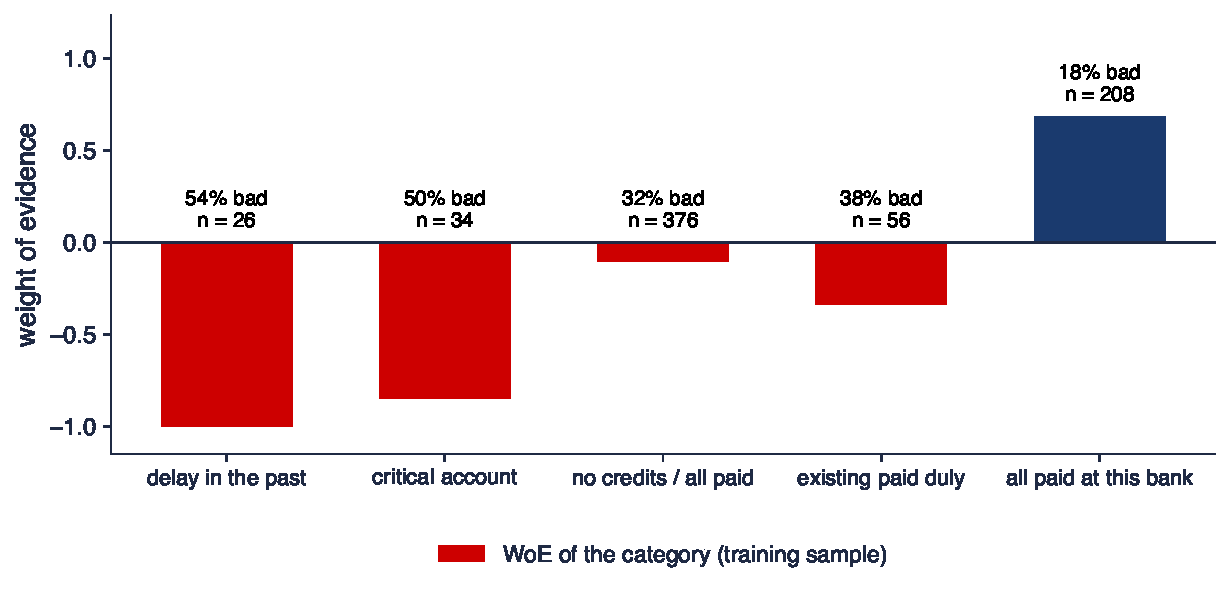
\includegraphics[width=0.96\textwidth,height=0.32\textheight,keepaspectratio]{ch12_sem_b1.pdf}
\end{center}
\vspace{-2mm}
\begin{center}
\tiny
\begin{tabular}{lrrrrrrr}
\toprule
& constant & checking account & credit history & purpose & savings & duration & years with the employer \\
\midrule
IV & & $0.591$ & $0.215$ & $0.205$ & $0.166$ & $0.159$ & $0.122$ \\
$\hat\beta$ & $-0.850$ & $-0.829$ & $-0.675$ & $-0.937$ & $-0.726$ & $-1.082$ & $-0.873$ \\
se & $0.095$ & $0.127$ & $0.206$ & $0.217$ & $0.246$ & $0.239$ & $0.265$ \\
\bottomrule
\end{tabular}
\end{center}
\begin{itemize}
    \item 6 variables with IV $\ge 0.1$; AUC: training $0.789$, test $0.801$, 95\% CI $[0.749, 0.854]$
    \item Interpretation: yes: a delay in the past (54\% bad) and a critical account (50\%) are the riskiest, all credits at this bank paid back duly (18\%) the safest; in the uncorrected UCI labels this safest group was called ``critical account''
\end{itemize}\sfmquantlet{Ch_12}{SFM_ch12_seminar}
\end{frame}

\begin{frame}{B2: Information Value of the Taiwan Data [Proposed]}
\itemsize{\footnotesize}
\begin{itemize}
\item \textbf{Question}: which kind of information predicts the default of a card holder: payment behaviour or personal data? Model: B1.
\item \textbf{Inputs}: Taiwan credit cards, 30\,000 clients; the same stratified 70/30 split
\item \textbf{Tasks}
\begin{enumerate}
    \item Compute the IV of \texttt{PAY\_0} and \texttt{PAY\_2} (repayment status in September and August; categories $-2$ to 3 or more), of \texttt{LIMIT\_BAL}, \texttt{PAY\_AMT1}, \texttt{BILL\_AMT1} and \texttt{AGE} (quintiles) and of \texttt{SEX}, \texttt{EDUCATION} and \texttt{MARRIAGE} (categories) on the training sample.
    \item Compute the default rate of each \texttt{PAY\_0} category.
    \item Rank the variables by IV and classify them with the rule of thumb.
    \item Interpretation: why is the last month's repayment status so much stronger than the personal data?
\end{enumerate}
\item \textbf{Report}: a table of nine IVs, six default rates and two sentences
\item Notebook: section B2
\end{itemize}
\end{frame}

\ifsolutions
\begin{frame}{B2: Solution [Proposed]}
\itemsize{\footnotesize}
\begin{center}
\scriptsize
\begin{tabular}{lrrrrrrrrr}
\toprule
& \texttt{PAY\_0} & \texttt{PAY\_2} & \texttt{LIMIT} & \texttt{PAY\_AMT1} & \texttt{EDUC.} & \texttt{AGE} & \texttt{MARR.} & \texttt{BILL\_AMT1} & \texttt{SEX} \\
\midrule
IV & $0.869$ & $0.564$ & $0.157$ & $0.148$ & $0.036$ & $0.013$ & $0.009$ & $0.009$ & $0.007$ \\
\bottomrule
\end{tabular}
\end{center}
\begin{itemize}
    \item Default rate by \texttt{PAY\_0}: $-2$: 13.3\%; $-1$: 16.9\%; 0: 12.9\%; 1: 33.1\%; 2: 69.0\%; 3 or more: 73.4\%
    \item \texttt{PAY\_0} and \texttt{PAY\_2}: strong; limit and payment: medium; education: weak; age, marital status, bill and sex: useless
    \item Interpretation: a client who is already two months late has most of the way to default behind him: behaviour measures the outcome almost directly, personal data only through averages
\end{itemize}\sfmquantlet{Ch_12}{SFM_ch12_seminar}
\end{frame}
\fi

\begin{frame}{B3: Validating the Scorecard [Solved]}
\itemsize{\footnotesize}
\begin{itemize}
\item \textbf{Question}: how good is the B1 scorecard on the test sample, and which cut-off should the bank use?
\item \textbf{Inputs}: the 300 test credits of B1 with their PDs; costs: 5 for an accepted bad, 1 for a rejected good
\item \textbf{Tasks}
\begin{enumerate}
    \item Build the confusion matrix at the cut-offs 0.5 and 1/6, with accuracy, TPR, FPR and the cost per applicant.
    \item Compute the AUC, the Gini, the accuracy ratio of the CAP curve and the KS statistic.
    \item Compute the Brier score, compare it with a constant PD of 30\%, and run the Hosmer--Lemeshow test with five groups.
    \item Draw the ROC curve with the two cut-offs and the calibration plot.
    \item Interpretation: which cut-off would you recommend to the bank?
\end{enumerate}
\item \textbf{Report}: a table of two confusion matrices, six statistics, the chart and two sentences
\item Notebook: section B3
\end{itemize}
\end{frame}

\begin{frame}{B3: Solution [Solved]}
\itemsize{\scriptsize}
\begin{center}
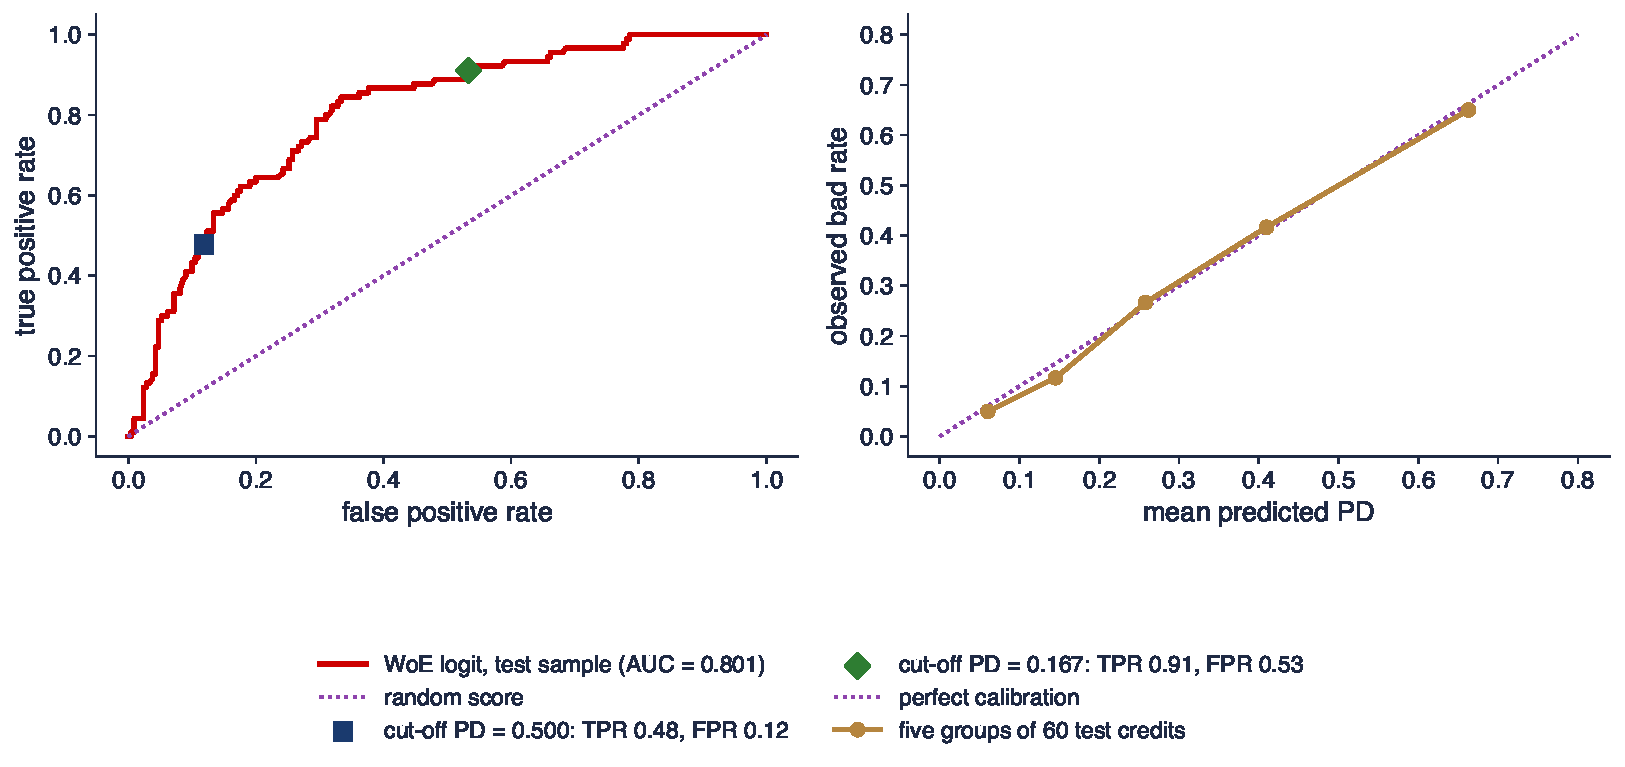
\includegraphics[width=0.96\textwidth,height=0.30\textheight,keepaspectratio]{ch12_sem_b3.pdf}
\end{center}
\vspace{-2mm}
\begin{center}
\tiny
\begin{tabular}{lrrrrrrrr}
\toprule
cut-off & TP & FN & FP & TN & accuracy & TPR & FPR & cost \\
\midrule
0.5 & 43 & 47 & 25 & 185 & $76.0\%$ & $47.8\%$ & $11.9\%$ & $0.867$ \\
1/6 & 82 & 8 & 112 & 98 & $60.0\%$ & $91.1\%$ & $53.3\%$ & $0.507$ \\
\bottomrule
\end{tabular}
\end{center}
\begin{itemize}
    \item AUC $= 0.801$, Gini $= 0.603$, AR $= 0.602$, KS $= 0.511$; Brier $= 0.162$ against $0.210$; HL $= 0.589$ (p $= 0.899$): no evidence of miscalibration
    \item Interpretation: the cut-off of 1/6: it rejects more applicants (64.7\%) but catches 91.1\% of the bads, and the cost falls from 0.867 to 0.507; accuracy is the wrong criterion when errors have different costs
\end{itemize}\sfmquantlet{Ch_12}{SFM_ch12_seminar}
\end{frame}

\begin{frame}{B4: Logit or LDA on the Taiwan Data? [Proposed]}
\itemsize{\footnotesize}
\begin{itemize}
\item \textbf{Question}: do the logit and Fisher's LDA differ in ranking or in calibration? Model: B3.
\item \textbf{Inputs}: Taiwan, 70/30 split; 13 standardised inputs: log limit, age, indicators of the September repayment status, number of late months, utilisation, log payments
\item \textbf{Tasks}
\begin{enumerate}
    \item Estimate a logit and an LDA on the training sample with the same inputs.
    \item Compute the test AUC of both and the DeLong test of equal AUCs.
    \item Compute the Brier score, the Hosmer--Lemeshow statistic (ten groups) and the mean PD of both, against the default rate.
    \item Compute the accuracy of the rule ``nobody defaults'' and of both models at the cut-off 0.5.
    \item Interpretation: is the LDA worse at ranking or at calibration?
\end{enumerate}
\item \textbf{Report}: one table and two sentences
\item Notebook: section B4
\end{itemize}
\end{frame}

\ifsolutions
\begin{frame}{B4: Solution [Proposed]}
\itemsize{\footnotesize}
\begin{center}
\scriptsize
\begin{tabular}{lrrrrrr}
\toprule
& AUC & Brier & HL & mean PD & accuracy (0.5) & TPR (0.5) \\
\midrule
logit & $0.777$ & $0.136$ & $40.7$ & $21.9\%$ & $81.9\%$ & $33.6\%$ \\
LDA & $0.778$ & $0.139$ & $282.5$ & $20.0\%$ & $81.9\%$ & $36.8\%$ \\
\bottomrule
\end{tabular}
\end{center}
\begin{itemize}
    \item DeLong: $z = -1.80$, p $= 0.072$; correlation of the log-odds $0.993$; test default rate 22.1\%; ``nobody defaults'': accuracy 77.9\%
    \item Both models beat the trivial rule by only 4.0 points of accuracy, but they catch about a third of the defaults
    \item Interpretation: at calibration: the ranking is the same (AUC equal at 5\%), but the LDA PDs are off (HL 282.5 against 40.7) because the inputs are dummies and skewed, far from Normal
\end{itemize}\sfmquantlet{Ch_12}{SFM_ch12_seminar}
\end{frame}
\fi

\begin{frame}{B5: From PDs to Capital [Solved]}
\itemsize{\footnotesize}
\begin{itemize}
\item \textbf{Question}: how much expected loss and Basel capital does the test portfolio of B1 carry, and how much does the prior correction matter?
\item \textbf{Inputs}: the 300 test credits of B1; EAD $=$ credit amount; LGD $= 45\%$; population bad rate 5\%; other retail exposures
\item \textbf{Tasks}
\begin{enumerate}
    \item Correct the PD of every credit from the sample rate of 30\% to the population rate of 5\%.
    \item Compute the expected loss of the portfolio, in DM and as a share of EAD, with and without the correction.
    \item Compute the IRB capital $K$ and the risk-weighted assets of the portfolio with the corrected PDs.
    \item Interpretation: why does the correction change the expected loss but not the AUC?
\end{enumerate}
\item \textbf{Report}: eight numbers and two sentences
\item Notebook: section B5
\end{itemize}
\end{frame}

\begin{frame}{B5: Solution [Solved]}
\itemsize{\footnotesize}
\begin{itemize}
    \item Shift of the log-odds: $\ln(0.05/0.95) - \ln(0.30/0.70) = -2.097$
    \begin{itemize}
        \item mean PD: 30.7\% in the sample scale, 7.3\% after the correction (median 4.2\%, maximum 54.4\%)
    \end{itemize}
    \item EAD 957\,819 DM; EL 41\,744 DM $=$ 4.4\% of EAD (without correction: 16.3\%)
    \begin{itemize}
        \item IRB capital $K$: 54\,542 DM $=$ 5.7\% of EAD; RWA 681\,771 DM, a risk weight of 71.2\%
    \end{itemize}
    \item The mean corrected PD is above 5\% because the correction is applied to the log-odds, not to the PD
    \item Interpretation: the correction adds the same constant to every log-odds: the order of the applicants, hence AUC, is unchanged, while every PD shrinks and EL falls from 16.3\% to 4.4\% of EAD
\end{itemize}\sfmquantlet{Ch_12}{SFM_ch12_seminar}
\end{frame}

\begin{frame}{B6: Fairness on the Taiwan Data [Proposed]}
\itemsize{\footnotesize}
\begin{itemize}
\item \textbf{Question}: does the logit of B4 treat men and women, and young and older clients, alike? Model: B5 and slide 5/5.
\item \textbf{Inputs}: Taiwan test sample (9000 clients); sex and age are not model inputs; approve the 75\% with the lowest PD
\item \textbf{Tasks}
\begin{enumerate}
    \item Compute the approval rate and the default rate of men and women, and of clients up to 25 years and older.
    \item Compute the approval rate of the good payers (equal opportunity) in each group.
    \item Compute the default rate among the approved clients of each group.
    \item Interpretation: which fairness criterion does the model come closest to satisfying?
\end{enumerate}
\item \textbf{Report}: one table and two sentences
\item Notebook: section B6
\end{itemize}
\end{frame}

\ifsolutions
\begin{frame}{B6: Solution [Proposed]}
\itemsize{\footnotesize}
\begin{center}
\scriptsize
\begin{tabular}{lrrrrr}
\toprule
& $n$ & default rate & approved & good payers approved & bad among approved \\
\midrule
men & 3\,574 & $24.7\%$ & $72.5\%$ & $83.2\%$ & $13.6\%$ \\
women & 5\,426 & $20.5\%$ & $76.6\%$ & $85.1\%$ & $11.6\%$ \\
age $\le$ 25 & 1\,153 & $25.8\%$ & $68.3\%$ & $80.0\%$ & $13.1\%$ \\
age $>$ 25 & 7\,847 & $21.6\%$ & $76.0\%$ & $85.0\%$ & $12.3\%$ \\
\bottomrule
\end{tabular}
\end{center}
\begin{itemize}
    \item Cut-off PD $= 23.5\%$; differences women $-$ men: approval $4.1$ points, good payers $2.0$; older $-$ young: $7.6$ and $5.0$ points
    \item Interpretation: equal opportunity: the gaps among good payers (2.0 and 5.0 points) are smaller than the gaps in approval (4.1 and 7.6), which mostly reflect the different default rates; parity would require different cut-offs by group
\end{itemize}\sfmquantlet{Ch_12}{SFM_ch12_seminar}
\end{frame}
\fi


%=============================================================================
\section{Part C: Open Questions and AI Critique}
%=============================================================================

\begin{frame}{C1: Does Gradient Boosting Beat the Logit? [Proposed]}
\itemsize{\footnotesize}
\begin{itemize}
\item \textbf{Question}: benchmarks report gains for flexible models \refLessmann; how large is the gain on the Taiwan data, and is it worth the loss of a simple scorecard?
\item \textbf{Inputs}: the inputs and the split of B4; models: B3, B4
\item \textbf{Tasks}
\begin{enumerate}
    \item Fit gradient boosting (scikit-learn, default settings) on the training sample.
    \item Compare its test AUC with the logit by the DeLong test, and compare the Brier scores.
    \item Compare the training and the test AUC of gradient boosting.
    \item Interpretation: is the gain large enough to replace the scorecard?
\end{enumerate}
\item \textbf{Report}: a table and a plan for a project
\item Notebook: section C1
\end{itemize}
\end{frame}

\ifsolutions
\begin{frame}{C1: Reference Analysis [Proposed]}
\itemsize{\footnotesize}
\begin{center}
\scriptsize
\begin{tabular}{lrrr}
\toprule
& test AUC & Brier & training AUC \\
\midrule
gradient boosting & $0.784$ & $0.134$ & $0.827$ \\
logit & $0.777$ & $0.136$ & $0.777$ \\
\bottomrule
\end{tabular}
\end{center}
\begin{itemize}
    \item DeLong: $z = 2.61$, p $= 0.009$: a significant but small gain (less than 0.01 in AUC); boosting also overfits more (training AUC 0.827)
    \item Project design: repeated cross-validation, cost-based and fairness measures by group, explanations of the boosting model, and the value of the gain in money (Lessmann et al.)
\end{itemize}\sfmquantlet{Ch_12}{SFM_ch12_seminar}
\end{frame}
\fi

\begin{frame}{C2: Audit an AI Answer [Proposed]}
\itemsize{\scriptsize}
\begin{itemize}
    \item A student asked an AI assistant to summarise the B1 scorecard. The answer:
    \item \aiprompt{(a) The AUC is 0.80, so the scorecard classifies 0.80 of the applicants correctly.}
    \item \aiprompt{(b) The Gini coefficient is AUC - 0.5 = 0.30.}
    \item \aiprompt{(c) An applicant with a PD of 30\% from this model has a 30\% chance of default at the bank.}
    \item \aiprompt{(d) With PDO = 20, a PD that halves from 20\% to 10\% adds exactly 20 points.}
    \item \aiprompt{(e) KS is the largest vertical gap between the score distributions of bads and goods.}
    \item \aiprompt{(f) LDA may only be used when every variable is Normally distributed.}
    \item Tasks
    \begin{itemize}
        \item 1. For each statement, say whether it is correct; if not, give the correct statement and, where possible, the correct number from the notebook (section C2).
        \item 2. Report: a list of six verdicts with one line of justification each.
    \end{itemize}
\end{itemize}
\end{frame}

\ifsolutions
\begin{frame}{C2: Solution [Proposed]}
\itemsize{\footnotesize}
\begin{itemize}
    \item (a) Wrong: AUC is the probability that a random bad has a higher PD than a random good; the accuracy at 0.5 is 76.0\%
    \item (b) Wrong: Gini $= 2\,\mathrm{AUC} - 1 = 0.603$
    \item (c) Wrong: the sample has 30\% bads, the bank about 5\%; after the prior correction the PD is 5.0\%
    \item (d) Wrong: PDO doubles the good:bad odds, not the PD: from 4:1 to 9:1 the score rises from 527.1 to 550.5, i.e.\ 23.4 points
    \item (e) Correct: $\max_s|F_{\text{bad}}(s) - F_{\text{good}}(s)|$
    \item (f) Wrong: Fisher's criterion needs no distribution; Normality with a common covariance is needed only for correct posterior PDs (B4)
\end{itemize}\sfmquantlet{Ch_12}{SFM_ch12_seminar}
\end{frame}
\fi


%=============================================================================
\section{Wrap-Up}
%=============================================================================

\begin{frame}{What You Should Take from Today}
\itemsize{\small}
\begin{itemize}
    \item A logit models the log-odds; $e^{\beta}$ is an odds ratio; the effect on PD is $p(1 - p)\beta$
    \item WoE and IV turn a table of goods and bads into evidence and a ranking of variables
    \item AUC counts correctly ordered pairs; Gini $= 2\,$AUC $- 1$; accuracy misleads when classes are imbalanced
    \item Choose the cut-off from the costs; correct oversampled PDs before any EL or capital
    \item An AI answer is a draft: check what AUC means, the Gini formula, the prior and the PDO scale
\end{itemize}
\end{frame}

\begin{frame}{After the Seminar}
\itemsize{\small}
\begin{itemize}
    \item Lecture 12 develops each topic of today: the Basel parameters, WoE and IV, logit and LDA, scorecards, validation, reject inference, fairness, Altman and Merton
    \item Try the [Proposed] tasks in the notebook; the solutions are discussed in class
    \item C1 can grow into a team project: cross-validated benchmark, costs and fairness by group
    \item Reading: \refFHH, Ch.~21--22; \refMVA, Ch.~14; \refSiddiqi
\end{itemize}
\end{frame}


%=============================================================================
\section{References}
%=============================================================================

\begin{frame}{References}
\itemsize{\tiny}
\begin{itemize}
    \item Basel Committee on Banking Supervision (2006). \href{https://www.bis.org/publ/bcbs128.htm}{International convergence of capital measurement and capital standards: a revised framework (comprehensive version)}. Bank for International Settlements.
    \item Brier, G.W. (1950). \href{https://doi.org/10.1175/1520-0493(1950)078<0001:VOFEIT>2.0.CO;2}{Verification of forecasts expressed in terms of probability}. \textit{Monthly Weather Review}, 78(1), 1--3.
    \item Cox, D.R. (1958). \href{https://doi.org/10.1111/j.2517-6161.1958.tb00292.x}{The regression analysis of binary sequences}. \textit{Journal of the Royal Statistical Society, Series B}, 20(2), 215--232.
    \item Default of Credit Card Clients [data set] (2009). \href{https://doi.org/10.24432/C55S3H}{UCI Machine Learning Repository}, CC BY 4.0.
    \item DeLong, E.R., DeLong, D.M., Clarke-Pearson, D.L. (1988). \href{https://doi.org/10.2307/2531595}{Comparing the areas under two or more correlated receiver operating characteristic curves: a nonparametric approach}. \textit{Biometrics}, 44(3), 837--845.
    \item Fisher, R.A. (1936). \href{https://doi.org/10.1111/j.1469-1809.1936.tb02137.x}{The use of multiple measurements in taxonomic problems}. \textit{Annals of Eugenics}, 7(2), 179--188.
    \item Franke, J., Härdle, W.K., Hafner, C.M. (2019). \href{https://doi.org/10.1007/978-3-030-13751-9}{\textit{Statistics of Financial Markets: An Introduction}}, 5th ed. Springer.
    \item Grömping, U. (2019). \href{http://www1.beuth-hochschule.de/FB_II/reports/Report-2019-004.pdf}{South German credit data: correcting a widely used data set}. Reports in Mathematics, Physics and Chemistry 4/2019, Beuth University of Applied Sciences Berlin.
    \item Hanley, J.A., McNeil, B.J. (1982). \href{https://doi.org/10.1148/radiology.143.1.7063747}{The meaning and use of the area under a receiver operating characteristic (ROC) curve}. \textit{Radiology}, 143(1), 29--36.
    \item Härdle, W.K., Simar, L. (2019). \href{https://doi.org/10.1007/978-3-030-26006-4}{\textit{Applied Multivariate Statistical Analysis}}, 5th ed. Springer.
    \item Hardt, M., Price, E., Srebro, N. (2016). \href{https://arxiv.org/abs/1610.02413}{Equality of opportunity in supervised learning}. \textit{Advances in Neural Information Processing Systems} 29; arXiv:1610.02413.
    \item Hosmer, D.W., Lemeshow, S. (1980). \href{https://doi.org/10.1080/03610928008827941}{Goodness of fit tests for the multiple logistic regression model}. \textit{Communications in Statistics -- Theory and Methods}, 9(10), 1043--1069.
    \item Lessmann, S., Baesens, B., Seow, H.-V., Thomas, L.C. (2015). \href{https://doi.org/10.1016/j.ejor.2015.05.030}{Benchmarking state-of-the-art classification algorithms for credit scoring: an update of research}. \textit{European Journal of Operational Research}, 247(1), 124--136.
    \item Siddiqi, N. (2006). \href{https://doi.org/10.1002/9781119201731}{\textit{Credit Risk Scorecards: Developing and Implementing Intelligent Credit Scoring}}. Wiley.
    \item South German Credit [data set] (2020). \href{https://doi.org/10.24432/C5QG88}{UCI Machine Learning Repository}, CC BY 4.0.
\end{itemize}
\end{frame}

\end{document}
